% spellchecker: disable
\usepackage{mathptmx}
\usepackage{setspace}
\usepackage{indentfirst}
\usepackage{fancyhdr}
\usepackage{titlesec}
\usepackage{tocloft}
\usepackage[nottoc]{tocbibind}
\usepackage[top=1in, bottom=1in, left=1.5in, right=1in, headheight=15pt]{geometry}

\setlength\parindent{2.5em}

\newcommand{\introduction}{
    \chapter{INTRODUCTION}
    \thispagestyle{fancy}
    \section{History and Theory}

Cosmic rays were discovered in 1911 by Victor Hess, for which he shared the 1936 Nobel Prize \cite{pleijel1936hessnobel}. Since his discovery, experiments have been conducted to determine the energy spectrum, arrival directions, and composition of cosmic rays.  The University of Utah has historically been involved in this research because of its proximity to the high deserts of the Great Basin. Among other things, the region has low light pollution and minimal cloud cover. Utah's experiments have primarily relied on the detection of nitrogen fluorescence with arrays of wide-angle telescopes. Two such experiments, Fly's Eye and High Resolution Fly's Eye (HiRes), were  instrumental in improving resolution at the high end of the energy spectrum \cite{abuzayyad2000hires, bird1994flyseye}. In 2007, HiRes was superseded by the Telescope Array Project, an international collaboration between the University of Utah, the University of Tokyo, and others. Telescope Array improves on the accuracy of HiRes by adding an array of ground-based scintillators \cite{stratton2012ta}.

It has been determined that most cosmic rays are hydrogen nuclei, with a small fraction of heavier nuclei like iron. It has also been found that energies obey a decreasing power law. In 1966, a theoretical maximum energy of \SI{5e19}{eV} was conjectured, leading to interest in the highest energy events \cite{greisen1966cutoff, zatsepin1966cutoff}. This theoretical maximum energy is known as the GZK cutoff, and results from the interaction of cosmic rays with the cosmic microwave background. The primary pathways are
\begin{equation}
\begin{aligned}
    \gamma + p &\rightarrow \Delta^+ \rightarrow p + \pi^0 \\
    \gamma + p &\rightarrow \Delta^+ \rightarrow n + \pi^+.
\end{aligned}
\end{equation}
In these interactions, a proton collides with a background photon, leading to the loss of energy through a $\pi^0$ or $\pi^+$. Over large distances, this and similar processes gradually reduce the energy of the proton to less than the threshold for the interaction. Interestingly, HiRes and other experiments have confirmed that the energy spectrum continues past the GZK cutoff. One of the primary goals of the Telescope Array project is determining the source of particles at this tail end of the spectrum. Below \SI{e18}{eV}, cosmic rays are believed to be of galactic origin and accelerated by supernova shock fronts \cite{abuzayyad2000hires}. Above this, one can only make educated guesses. If particles are contained by a magnetic field during their acceleration, there are restrictions on the size and field strength of accelerators. These restrictions can be summarized in a Hillas Plot, shown in Figure \ref{fig:hillas}. 

The decreasing power law of cosmic ray flux creates a problem for high energy experiments. The flux in this regime is very low (on the order of one per square kilometer per century), so direct detection is impractical. Fortunately, ultra high energy rays interact with the atmosphere and can be indirectly observed by distant detectors. High energy cosmic rays initiate a cascade of photons and charged particles (mostly fermions) upon entering the atmosphere. This shower multiplies through an alternating sequence of Bremsstrahlung and pair creation \cite{abuzayyad2000hires}. Shower particles interact with atmospheric nitrogen, producing fluorescence which can be observed by a sensitive detector. The slant depth of the fluorescence peak increases with the energy of the primary, with ultra high energy cascades typically peaking between \num{725} and \SI{890}{g/cm^2} \cite{abuzayyad2000hires}. The Great Basin, at a depth of roughly \SI{860}{g/cm^2}, is ideally situated to view these events.

\begin{figure}[ht]
    \label{fig:hillas}
    \centering
    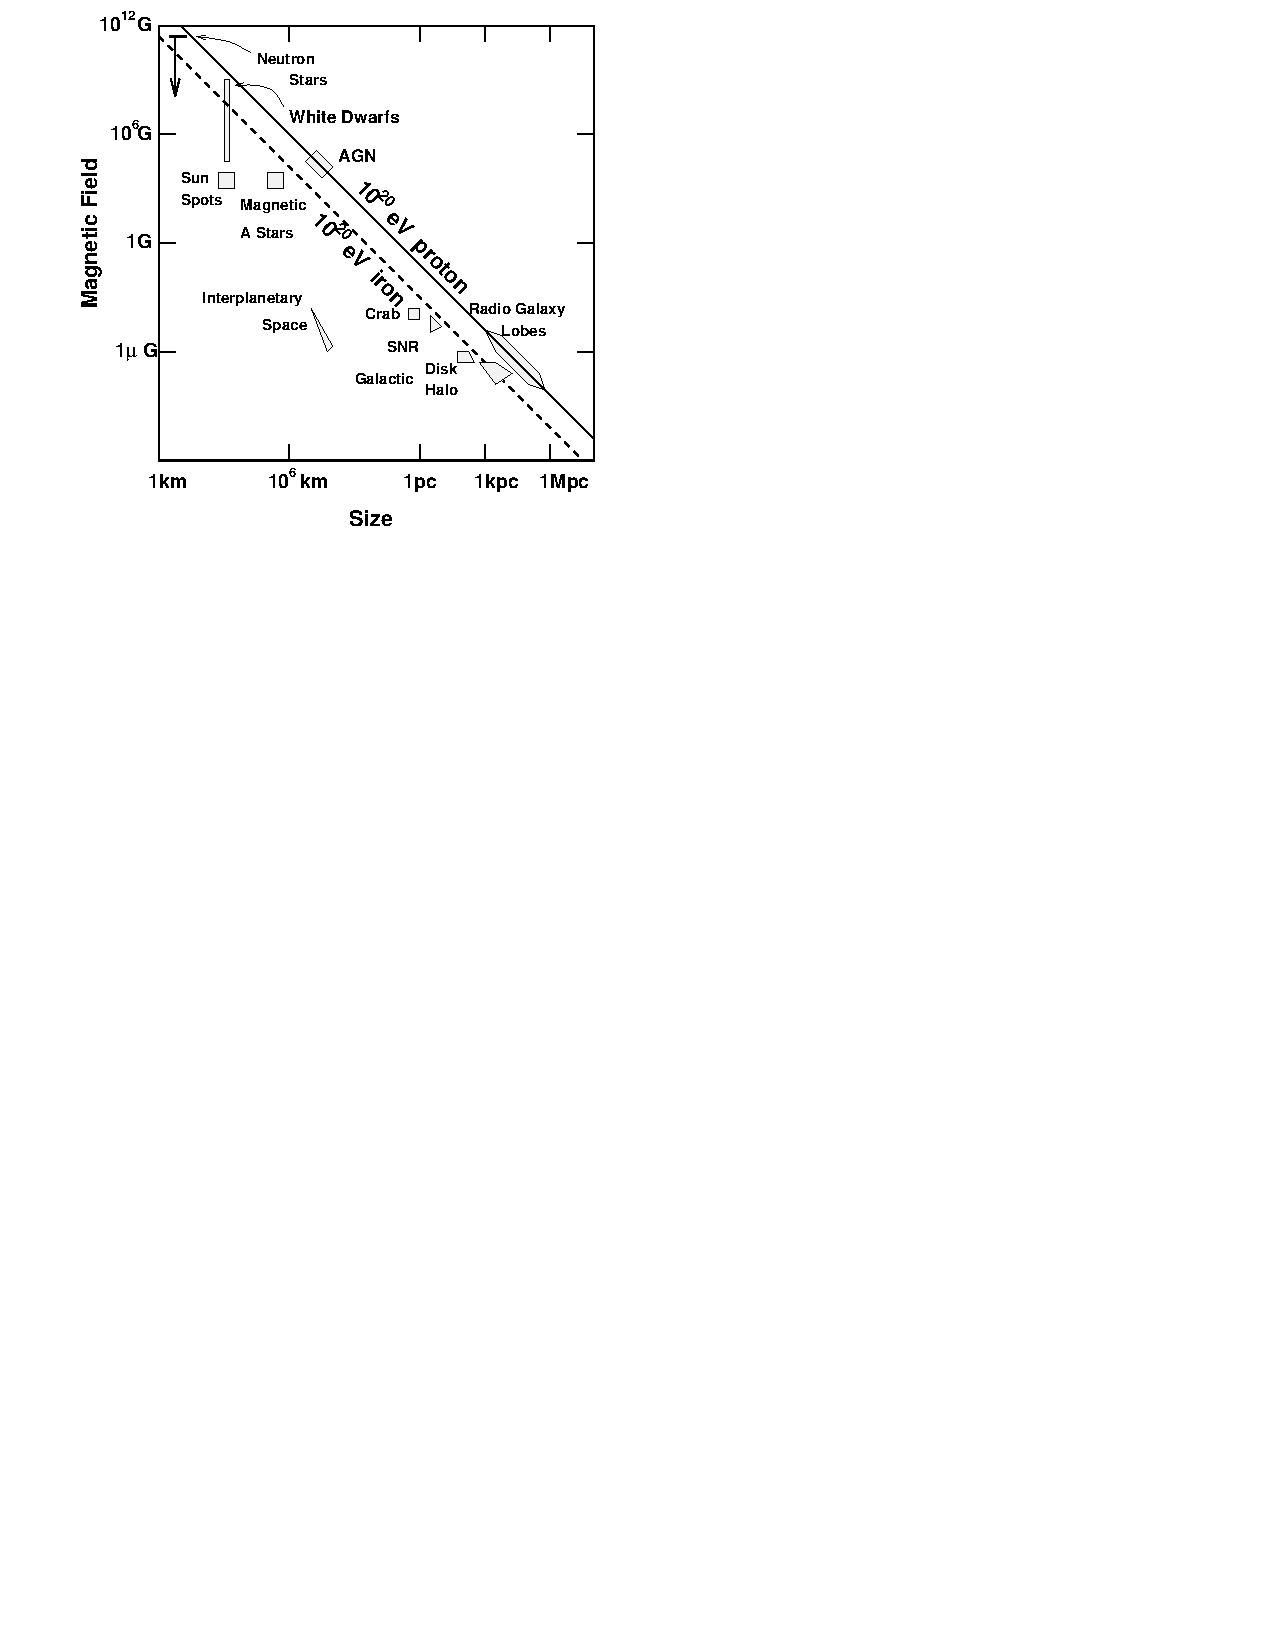
\includegraphics[width=0.8\textwidth]{HillasPlot}
    \caption{A Hillas Plot, taken from Yoshida \cite{yoshida1998uhecr}. Structures of larger size and stronger magnetic field can accelerate particles to higher energies. Candidates for the acceleration of \SI{e20}{eV} protons are radio galaxy lobes and active galactic nuclei.}
\end{figure}

Although cascades' individual particle interactions are well understood, their overall development and light production are too complex to be derived analytically. This precludes the possibility of directly determining properties of a cosmic ray from its cascade's light production. Simulated values and phenomenological models are used in place of analytic methods. A 1977 paper proposed a parameterization for the number of particles in a shower as a function of atmospheric depth, $X$ \cite{gaisser1977profile}. This parameterization, the Gaisser-Hillas profile, has become a standard in cosmic ray physics.
\begin{equation} \label{eq:gaisser_hillas}
    N(X) = N_\text{max} \left(\frac{X - X_0}{X_\text{max} - X_0}\right)
        ^{\frac{X_\text{max} - X_0}{\lambda}} 
        \exp{\left(\frac{X_\text{max} - X}{\lambda}\right)}
\end{equation}
$N_\text{max}$ is the maximum size of the shower, $X_0$ the depth of the first interaction, and $X_\text{max}$ the depth of the shower maximum. $\lambda$ is a scaling factor usually taken as $\SI{70}{g/cm^2}$. $N_\text{max}$, $X_0$, and $X_\text{max}$ depend straightforwardly on the energy of the primary particle (see Section \ref{sec:shower_gen}). In addition to knowing the number of particles in a shower, it is valuable to know distributions of their properties. CORSIKA simulates the interactions within a shower and records particle energies and velocities at each step \cite{heck1998corsika}. Various models of the CORSIKA data have been made, and are used with the Gaisser-Hillas profile to understand average particle behavior. For instance, Nerling gives a parameterization of the distribution of electron energies as a function of shower age \cite{nerling2006electron}.

Such models are useful when simulating shower light production. There are two main emission mechanisms. The first, fluorescence, occurs when shower particles excite atmospheric nitrogen. This emission is isotropic and heaviest in the UV. A parameterization of fluorescence production is given by Kakimoto as a function of the shower's atmospheric energy deposit \cite{kakimoto1996yield}. The second emission mechanism, Cherenkov radiation, can be thought of as a ``shock front'' resulting when particles exceed the speed of light in air, $c / n$. Unlike fluorescence, Cherenkov radiation is produced in a cone around each shower particle's direction. The dimensions of the cone are determined solely by the particle's speed and the value of $c / n$. In a cascade, individual cones must be convolved with the distribution of particle directions. Models of Cherenkov production and angular distributions are given by Nerling \cite{nerling2006electron}.

\section{Geometric Reconstruction} \label{sec:intro_recon}

Correctly determining a shower's energy is only possible with an accurate geometric reconstruction. In this work, we investigate a hybrid technique to reduce the cost of obtaining this geometric accuracy. Current algorithms differ depending on whether the detector is monocular (only one ground station) or stereo (multiple stations). In both cases, each station performs a fit of the shower-detector plane (defined as containing both the shower axis and the detector). In stereo mode, the shower axis is found by intersecting two or more shower-detector planes. This typically gives the direction to within a couple of degrees. In monocular mode, the shower's distance and angle are found by fitting a function of  photon arrival times. Using Figure \ref{fig:mono}, one can find the expected arrival time of the $i^\text{th}$ recorded photon. We define the impact parameter $R_p$ to be the distance of closest approach, and $t_0$ to be the time when the shower reaches this closest distance. $\psi$ is the angle of the axis within the shower-detector plane.
\begin{equation} \label{eq:time_prof}
\begin{aligned}
    t_i &= t_0 - \frac{R_p}{c \tan{\theta_i}} + \frac{R_p}{c \sin{\theta_i}} \\[4pt]
        &= t_0 + \frac{R_p}{c} \left(\frac{1 - \cos{\theta_i}}{\sin{\theta_i}}\right) \\[4pt]
        &= t_0 + \frac{R_p}{c} \tan{\left(\frac{\pi - \psi - \chi_i}{2}\right)}
\end{aligned}
\end{equation}
This function is difficult to fit because $R_p$, $\psi$, and $t_0$ are correlated free parameters. An overestimate of $\psi$ is typically accompanied by an overestimate of $R_p$ and an underestimate of $t_0$. In addition, the visible portion of the tangent is nearly linear for most showers, hiding structural information. Kidd explores the limitations of monocular reconstruction, and estimates $\sigma_{Rp} \sim L^{-5/2}$, where $L$ is the angular size of the track \cite{kidd1997properties}.

\begin{figure}[ht]
    \label{fig:mono}
    \centering
    \frame{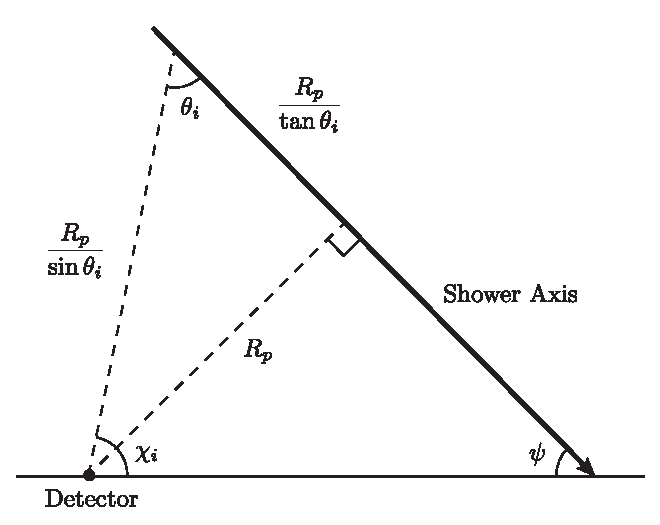
\includegraphics[width=0.8\textwidth]{MonoReconstruction}}
    \caption{The geometry of a monocular reconstruction. $\theta_i$ and $\chi_i$ change for each point along the shower axis, whereas $R_p$ and $\psi$ are properties of the entire shower.}
\end{figure}

Monocular experiments are desirable for their simplicity and lower cost, but as seen, come with compromises in data quality. We propose a technique which uses Cherenkov radiation to improve the accuracy of monocular reconstruction. Because Cherenkov radiation is collimated along the shower axis, most strikes the ground near the shower core, where some is reflected back into the detector. The reflection point lies along the shower axis, and can be used to reduce the number of parameters in the monocular fit from three to two. This reduction makes use of the following relationship:
\begin{equation} \label{eq:ckv_relation}
    R_p = d \sin(\psi + \alpha).
\end{equation}
$d$ is the distance from the detector to the ground reflection point, and $\alpha$ the angle of this point below the horizon. In this work, we investigate the feasibility of this Cherenkov-assisted reconstruction. Using simulations, we determine whether the Cherenkov reflection gives a strong signal and whether it can be used to improve accuracy.

\begin{figure}[!ht]
    \label{fig:hybridrecon}
    \centering
    \frame{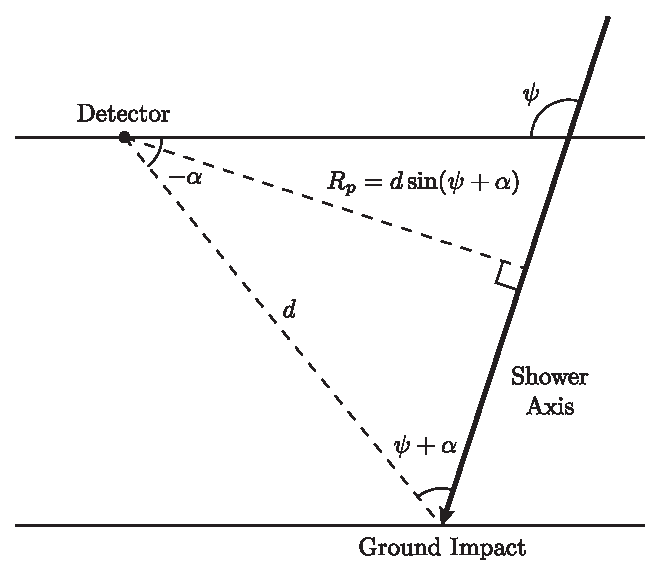
\includegraphics[width=0.8\textwidth]{CherenkovReconstruction}}
    \caption{The geometry of a Cherenkov-assisted reconstruction, showing the fixed relationship between $R_p$ and $\psi$.}
\end{figure}

The quality of the hybrid Cherenkov reconstruction depends considerably on the height $h$ of the detector above the ground. Assuming a Lambertian model of ground reflection, the amount of Cherenkov light seen is proportional to $\sin{\alpha}$. This means that the backscattering signal is nearly proportional to the detector height. In addition, the error in $d$ is inversely related to $h$ according to
\begin{equation} \label{eq:ground_err}
    \Delta d \approx \frac{d \Delta \alpha}{\sin{\alpha}} = \frac{d^2 \Delta \alpha}{h}.
\end{equation}
$\Delta \alpha$ is the angular size of a single pixel, and $\Delta d$ is the ground distance covered by a single pixel, equivalent to the error in $d$. The linear dependence on pixel size highlights the need for a high resolution detector. To achieve this, we use an f/1 Schmidt camera, which is a high-speed, wide-angle telescope with low spherical aberration. Both the focal surface and primary mirror are spherical, and in our simulation are given radii of \SI{1}{m} and \SI{2}{m}. A corrector plate is placed at the stop \cite{malacara2004optics}. As shown in Figure \ref{fig:schmidt}, the corrector has thick sections in the middle (a quadratic term), and near the edge (a quartic term). Because of the lens's large size, the decision was made to remove the central quadratic portion. This leaves a ring at the outside of the stop which could be assembled in slices. The detector height is varied throughout the simulation (see Section \ref{sec:results}).

\begin{figure}[!ht]
    \label{fig:schmidt}
    \centering
    \frame{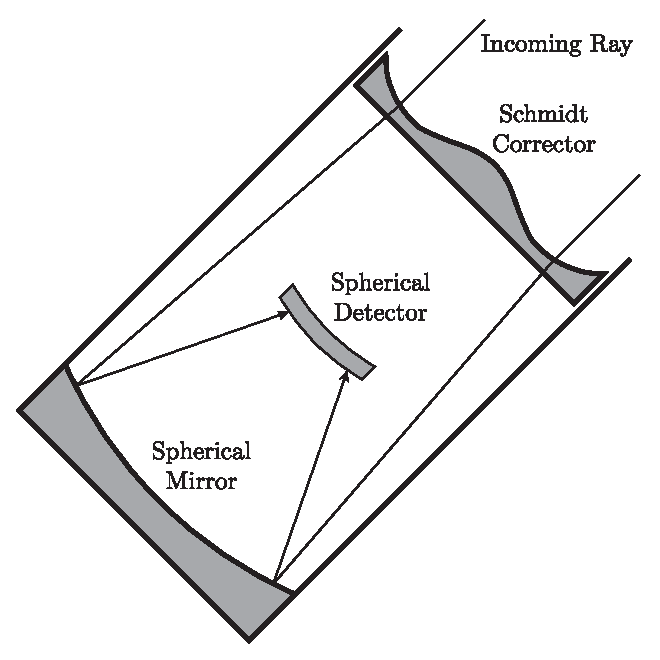
\includegraphics[width=0.8\textwidth]{SchmidtCamera}}
    \caption{A Schmidt camera. In this experiment, the thick inner portion of the corrector has been removed. The corrector deflects incoming rays to improve the camera's spherical symmetry.}
\end{figure}

\section{Summary of Simulation} \label{sec:sim_summary}

Simulating individual showers can give an idea of the typical appearance of the Cherenkov reflection and the quality of the hybrid reconstruction. More robust conclusions can be drawn from a Monte Carlo, which simulates a large number of representative showers. For all of these showers, a Cherenkov-assisted reconstruction is attempted and its accuracy is compared to the traditional method. Relative accuracies can be used to determine the range of parameters (e.g. angle or energy) in which the Cherenkov reconstruction gives an improvement. Each Monte Carlo iteration consists of three steps: the statistical generation of a shower, a simulation of its detection, and an attempt at reconstruction. The details of each of these steps are given in Section \ref{sec:methods}. When examining a specific shower energy and geometry the statistical generation step is eliminated. When probing the overall performance of the detector in a Monte Carlo, the generation-simulation-reconstruction process is repeated many times. Random shower energies are chosen from a power law and are used to determine Gaisser-Hillas parameters based on relations from Abuzayyad \cite{abuzayyad2000hires}. A direction and point of closest approach are randomly chosen. Using its direction, the shower is traced back from its closest approach to a starting point higher in the atmosphere.

From this starting point, the shower iterates through discrete steps of equal atmospheric thickness. At each step, the size of the shower is calculated from the Gaisser-Hillas profile and combined with parameterizations from Kakimoto and Nerling to obtain fluorescence and Cherenkov photon numbers \cite{gaisser1977profile,kakimoto1996yield,nerling2006electron}. These numbers are adjusted to account for the varying perspective and distance of the detector. Captured fluorescence photons are traced directly from the shower core to the detector. Cherenkov photons are given random directions around the shower axis, traced to their ground collision point, and reflected back into the detector. Both fluorescence and Cherenkov rays are traced through the detector optics to the pixel array, where they are binned and recorded.

This results in a three-dimensional histogram with a binned time series for each pixel on an x-y grid. If reconstruction were attempted immediately on this data set, it would usually be successful, regardless of the distance or brightness of the shower. Because this wouldn't give information about the real limits of the detector, background noise is first added to each time series. The noise in a particular bin is randomly sampled from a Poisson distribution. The mean noise level is then subtracted from the signal, and a bleeding algorithm is used to find chunks of non-noise signals. Triggering logic is applied to determine whether the track is sufficiently large and bright to attempt a reconstruction. If the detector is triggered, the shower-detector plane is fit and a standard monocular reconstruction is performed. A hybrid reconstruction is attempted if the Cherenkov reflection is sufficiently bright and within the field of view.}
\newcommand{\methods}{
    \chapter{METHODS}
    \thispagestyle{fancy}
    \section{Implementation}

\subsection{Project Structure}

The simulation is implemented in C++. Implementation details will only be covered briefly here; the interested reader can visit \url{github.com/mattdutson/cherenkov_simulator} to view the source code. Any parameter values, where not explicitly given here, can be found in \texttt{Utility.h} or \texttt{Config.xml}. The project relies on three external libraries. CERN's ROOT libraries (\url{root.cern.ch}) are used for vector operations, coordinate transformations, fitting, and eigenvector finding among other things. The Boost libraries (\url{boost.org}) expand the core functionality of the C++ standard library. We only use the \texttt{property\_tree} class, which parses XML files into a hierarchical structure. Google Test (\url{github.com/google/googletest}) is used both to perform unit testing and to conveniently simulate individual shower cases. ROOT comes with a set of dynamic libraries which need to be referenced via environment variable during execution. Boost is header-only, and Google Test is built as a subdirectory of the project.

The top-level project directory, \texttt{cherenkov\_simulator}, contains the main executable, the XML configuration file, and subdirectories \texttt{cherenkov\_test} and \texttt{cherenkov\_lib}. \texttt{cherenkov\_test} contains unit tests and sample showers. Individual tests and showers can be run via command-line arguments to the \texttt{cherenkov\_test} executable (see the Google Test documentation). \texttt{cherenkov\_lib} implements all simulation, reconstruction, and Monte Carlo methods. It is compiled as a static library and linked to the other two executables.

\subsection{Configuration and Operation}

Simulation parameters are split between the executable and configuration file. Physical constants and most model parameters are hard coded in \texttt{Utility.h}. These values are unlikely to change from run to run. It's both cleaner and faster to hard code them than to re-parse on each execution. Other more variable parameters are stored in \texttt{Config.xml}. Among other things, they define the behavior of the simulation, the geometry of the detector, and noise removal thresholds. Running the main executable, \texttt{cherenkov\_simulator}, performs the Monte Carlo generation-simulation-reconstruction cycle. The first command-line argument is mandatory and specifies the path of the output file. If the user specified the output as \texttt{MonteCarlo}, then \texttt{MonteCarlo.root} and \texttt{MonteCarlo.csv} would be written to the current directory. The ROOT file contains plots of each shower, and the CSV summarizes the results of all reconstructions. The second argument is optional, and specifies a configuration file other than the default \texttt{Config.xml}. The third argument is also optional and sets the random number seed (an unsigned integer). This allows for repeatability between runs.

\subsection{Class Structure}
The following list summarizes the major classes defined in the implementation of \texttt{cherenkov\_lib}. \texttt{PhotonCount} is defined in \texttt{DataStructures.h}, and \texttt{Ray} and \texttt{Shower} are defined in \texttt{Geometric.h}. The remaining classes are defined in files which match their names.
\begin{itemize}
    \item \texttt{Ray}: A photon with a three-dimensional position and velocity. Keeps track of the current time, which is updated when the photon moves. Implements methods for reflection, refraction, and propagation.
    \item \texttt{Shower}: An extension of \texttt{Ray} which stores the primary particle's energy along with Gaisser-Hillas parameters. Implements methods for age, size, and atmospheric depth.
    \item \texttt{PhotonCount}: A three-dimensional array which is incremented in a certain (x, y, t) bin whenever a photon is detected. Stores linear and angular pixel size information, which is used when determining a pixel's direction with respect to the detector axis. A \texttt{PhotonCount::Iterator} can be used to move through the circular collection of valid pixels.
    \item \texttt{Simulator}: Simulates the development and detection of a shower. All member functions but the constructor are \texttt{const}. The constructor takes the parsed configuration file and stores required parameters as members.
    \item \texttt{Reconstructor}: Used for reconstructing a shower from the \texttt{PhotonCount} data produced by \texttt{Simulator}. Implements methods for the addition and subsequent filtering of noise. Similar to \texttt{Simulator} in structure.
    \item \texttt{MonteCarlo}: Used for performing the Monte Carlo cycle and generating random showers. Similar to \texttt{Simulator} in structure, but has a member \texttt{Simulator} and \texttt{Reconstructor}.
    \item \texttt{Analysis}: Defines a suite of static methods which can be used to plot and analyze the data in a \texttt{PhotonCount}.
    \item \texttt{Utility}: Implements miscellaneous static methods and defines hard-coded constants.
\end{itemize}
There are a handful of minor classes not listed here, most used as convenience wrappers for method parameters.

\section{Coordinate Systems and Surroundings} \label{sec:atmosphere}

The simulation uses three reference frames: the world frame, the detector frame, and the shower-detector frame. In all three, the telescope's center of curvature is the origin. This simplifies ray tracing and reduces transformations between frames to a rotation. In the world frame, the z-axis is perpendicular to the surface of the Earth. The y-axis is found by rotating the detector axis downward until it's horizontal, and the x-axis is given by the right hand rule. In the detector frame, the z-axis points along the detector axis, and the x-axis is shared with the world frame. The y-axis is again given by the right hand rule and typically points below the horizon. During reconstruction, a shower-detector plane is determined. The normal to this plane is the z-axis of the shower-detector frame. The x-axis must be in the world's x-y plane, and the y-axis is given by the right hand rule.

The ground is a simple plane with geometry defined in the configuration file. The user specifies, in the world frame, the plane's normal vector and a point which fixes its position. The normal vector doesn't necessarily align with the direction of atmospheric variation, which is $(0, 0, 1)$. The atmosphere is approximated with an exponential model. To derive this, we start with the ideal gas equation and a differential equation for pressure variation.
\begin{align}
    P &= \frac {\rho RT}{M} \\
    \text{d}P &= -\rho g \text{d}h
\end{align}
$M$ is the gas's molar mass, and $R$ is the ideal gas constant. If the temperature of the atmosphere is assumed constant, then the ideal gas equation gives a direct proportionality between $\rho$ and $P$, leading to the following solution:
\begin{equation}
\begin{aligned}
    \rho &= \rho_0 e^{-gMh / RT} \\
         &= \rho_0 e^{-h / H}.
\end{aligned}
\end{equation}
$\rho_0$ is the density at sea level, and $h$ is the elevation. $H$ is the ``scale height.'' Although it could be calculated directly by finding the atmosphere's molar mass and fixing a constant temperature, we chose to calculate it based on the atmospheric pressure at sea level.

\section{Random Shower Generation} \label{sec:shower_gen}

As discussed in Section \ref{sec:sim_summary}, each iteration of the Monte Carlo simulation begins with the random generation of a shower. This involves choosing a random geometry, energy, and set of Gaisser-Hillas parameters. The shower is first given a zenith angle $\theta$, which is distributed as $\cos{\theta}$ between zero and $\pi/2$. The shower is also given an azimuthal angle $\phi$, uniformly distributed between zero and $2\pi$. Together, these two angles completely define the direction of the shower. Recall that the impact point is the shower's closest approach to the detector (not to be confused with the ground reflection point). The allowed impact points lie on a disk centered at the detector and perpendicular to the shower direction. Points on the disk can be specified with polar coordinates $\beta$ and $R_p$. $\beta$ is distributed uniformly between zero and $2\pi$, and $R_p$ is chosen from a linear distribution between $R_\text{min}$ and $R_\text{max}$. $R_\text{min}$ = \texttt{impact\_min} and $R_\text{max}$ = \texttt{impact\_max} are defined in the configuration file. From the impact point, the shower is traced back to a starting point at depth $X_s$ = \texttt{start\_tracking}. Because the exponential atmosphere extends to infinity, $X_s$ must be positive. The starting height is found by integrating the atmospheric density from infinity and accounting for the zenith angle of the shower.
\begin{equation}
    h_s = -H \ln{\left(\frac{X_s \cos{\theta}}{\rho_0 H}\right)}
\end{equation}
Once the height is known, the starting $x$ and $y$ can be extrapolated using the shower direction and impact point.

\begin{figure}[!ht]
    \centering
    \frame{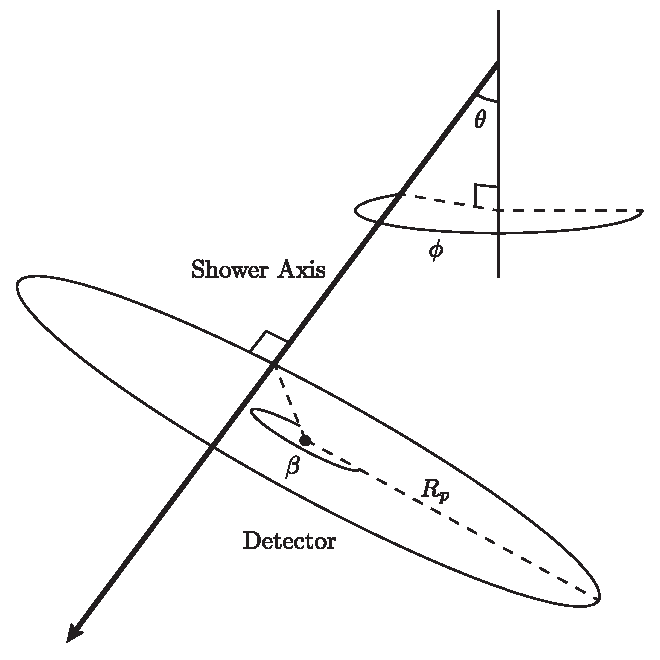
\includegraphics[width=0.8\textwidth]{ShowerGeneration}}
    \caption{Choosing the random geometry of a shower.}
\end{figure}

The primary energy is chosen from a power law, which has a slope, minimum, and maximum defined in the configuration file. The Gaisser-Hillas parameters (see Equation \ref{eq:gaisser_hillas}) can be calculated directly from the energy. $X_0$ is assigned a constant value of \SI{-70}{g/cm^2}. Although not physically realizable in an exponential atmosphere, this value gives a well-behaved Gaisser-Hillas function. The remaining parameters are calculated from the energy using
\begin{gather}
    X_\text{max} = 725 + 55.0 (\log_{10}(E) - 18.0) \\
    N_\text{max} = E / 1.3 \times 10^9.
\end{gather}
These expressions assume a proton primary and units of \si{eV} and \si{g/cm^2} \cite{abuzayyad2000hires}.

\section{Light Production} \label{sec:light_prod}

\subsection{Fluorescence Yield} \label{sec:fluorescence}

Once a shower has been initialized, it is stepped along its axis. At each step, the simulation determines the number of fluorescence and Cherenkov photons observed. Kakimoto gives the following parameterization of the number of fluorescence photons produced by a shower per unit per slant depth \cite{kakimoto1996yield}.
\begin{equation} \label{eq:fluorescence}
    Y_\text{fl} = \frac{\text{d}E / \text{d}X}{(\text{d}E / \text{d}X)_{\SI{1.4}{MeV}}}
        \left(\frac{A_1}{1 + \rho B_1 \sqrt{T}} + \frac{A_2}{1 + \rho B_2 \sqrt{T}}\right)
\end{equation}
The constants are given as $A_1 = \SI{890}{cm^2/g}$, $A_2 = \SI{550}{cm^2/g}$, $B_1 = \num{1.85e3}$ \si{cm^3/g.K^{1/2}}, and $B_2 = \SI{6.50e3}{cm^3/g.K^{1/2}}$. $\text{d}E / \text{d}X$ is the energy deposit, the rate per slant depth at which the shower loses energy to the atmosphere. $(\text{d}E / \text{d}X)_{\SI{1.4}{MeV}}$ is the energy deposit of a single \SI{1.4}{MeV} electron, given as \SI{1.6}{MeV.cm^2/g}. Kakimoto's original parameterization of $Y_\text{fl}$ came with a factor of $\rho$, and was expressed per unit distance. Dividing by $\rho$ gives the formula in units of slant depth instead.

Nerling gives a parameterization of the energy deposit as a function of shower age \cite{nerling2006electron}. Age is a unitless quantity defined as $s = 3X / (X + 2X_\text{max})$.
\begin{gather} \label{eq:deposit}
    \diff{E}{X}(X) = \alpha_\text{eff}(X, E > E_\text{cut}) \cdot N(X, E > E_\text{cut}) \\
    \alpha_\text{eff}(s) = \frac{c_1}{(c_2 + s)^{c_3}} + c_4 + c_5 \cdot s
\end{gather}
$\alpha_\text{eff}$ is the effective ionization loss rate, representing the energy deposit of a single particle. The constants are given as $c_1 = \num{3.90883}$, $c_2 = \num{1.05301}$, $c_3 = \num{9.91717}$, $c_4 = \num{2.41715}$, and $c_5 = \num{0.13180}$. These values give $\alpha_\text{eff}$ in units \si{MeV.cm^2/g}. Note that both terms in Equation \ref{eq:deposit} depend on $E_\text{cut}$, a simulation cutoff used by CORSIKA. The formula for $\alpha_\text{eff}$ assumes a cutoff of \SI{1}{MeV}. For reasons discussed in Section \ref{sec:cherenkov}, it is sufficient to use the cutoff-independent Gaisser-Hillas parameterization in place of $N(X, E > E_\text{cut})$. With this, the fluorescence yield obtains its final form.
\begin{equation} \label{eq:fluor}
    Y_\text{fl} = \frac{\alpha_\text{eff}(s) \cdot N(X)}{(\text{d}E / \text{d}X)_{\SI{1.4}{MeV}}} 
        \left(\frac{A_1}{1 + \rho B_1 \sqrt{T}} + \frac{A_2}{1 + \rho B_2 \sqrt{T}}\right)
\end{equation}

\subsection{Cherenkov Yield} \label{sec:cherenkov}

The Cherenkov yield for an individual shower electron varies with its energy. Nerling gives the following parameterization of the Cherenkov yield of a single electron \cite{nerling2006electron}:
\begin{equation}
    Y_\text{cv}(h, E) = \frac{2 \pi \alpha Z^2}{\rho(h)} 
        \int^{\lambda_2}_{\lambda_1} \left(1 - \frac{1}{n^2(h, \lambda) \beta^2}\right) 
        \frac{\text{d} \lambda}{\lambda^2}
\end{equation}
$\alpha$ is the fine structure constant, $Z = 1$, $n$ is the atmospheric index of refraction, and $\beta = v / c$. $(\lambda_1, \lambda_2)$ is the range of wavelengths to which the detector is sensitive, something like 300-400 \si{nm}. Because the dependence of $n$ on wavelength is small and $n \approx 1$, the yield can be simplified. We define $\delta(h) = 1 - n(h)$.
\begin{equation}
\begin{gathered}
    1 - (n \beta)^{-2} \approx 2 \delta - \frac{m^2 c^4}{E^2} \\
    Y_\text{cv}(h, E) \approx \frac{2 \pi \alpha Z^2}{\rho(h)} 
        \left(\delta(h) - \frac{m^2 c^4}{E^2}\right)
        \left(\frac{1}{\lambda_1} - \frac{1}{\lambda_2}\right)
\end{gathered}
\end{equation}
The Cherenkov yield for the entire shower is calculated by averaging the single particle yield over the electron energy spectrum, then multiplying that expectation value by the total number of electrons. This gives the total number of Cherenkov photons produced per slant depth.
\begin{equation} \label{eq:ckv_yield}
    \diff{N_\gamma}{X} = N(X) \int^{\infty}_{\ln{E_\text{thr}}} 
        Y_\text{cv}(h, E) f_e(s, E) \text{d} \ln{E}
\end{equation}
$E_\text{thr} = m_e c^2 / \sqrt{2 \delta}$ is the threshold below which an electron will not produce Cherenkov radiation. Nerling gives a parameterization of the electron energy spectrum as a function of shower age \cite{nerling2006electron}.
\begin{gather}
    f_e(s, E) = a_0 \cdot \frac{E}{(E + a_1)(E + a_2)^s} \\
    \begin{aligned}
        a_0 &= k_0 \exp(k_1 \cdot s + k_2 \cdot s^2) \\
        a_1 &= \num{6.42522} - \num{1.53183} \cdot s \\
        a_2 &= \num{168.168} - \num{42.1368} \cdot s
    \end{aligned}
\end{gather}
$E$ is assumed to have units of \si{MeV}. The choice of the normalization constant $a_0$ depends on the CORSIKA cutoff energy. It is chosen such that
\begin{equation}
    \int^{\infty}_{\ln{E_\text{cut}}} f_e(X, E) \text{d} \ln{E} = 1.
\end{equation}
As for the fluorescence yield, we assume $E_\text{cut} = \SI{1}{MeV}$. This cutoff gives  $k_0 = \num{0.145098}$, $k_1 = \num{6.20114}$ , and $k_2 = \num{-0.596851}$. Equation \ref{eq:ckv_yield} must be integrated numerically. To improve the speed and robustness of this integration, its upper limit is set to the natural log of the total shower energy. The spectrum remains well normalized under this approximation. 

There is a subtlety to be addressed regarding the CORSIKA cutoff energy. The normalization of the electron energy spectrum depends on the cutoff, which means that our Cherenkov yield differs depending on what we choose as the cutoff. We could correct for this by using $N_\text{ch}(E > E_\text{cut})$ instead of the Gaisser-Hillas number. Figure \ref{fig:corsika_cut} demonstrates the dependence of $N_\text{max}$ on the cutoff energy, where a cutoff of zero corresponds to the unmodified Gaisser-Hillas parameterization \cite{nerling2006electron}. Due to the small fractional change from zero to $E_\text{cut} = \SI{1}{MeV}$, the Gaisser-Hillas value is used without correction.

\begin{figure}[!ht]
    \label{fig:corsika_cut}
    \centering
    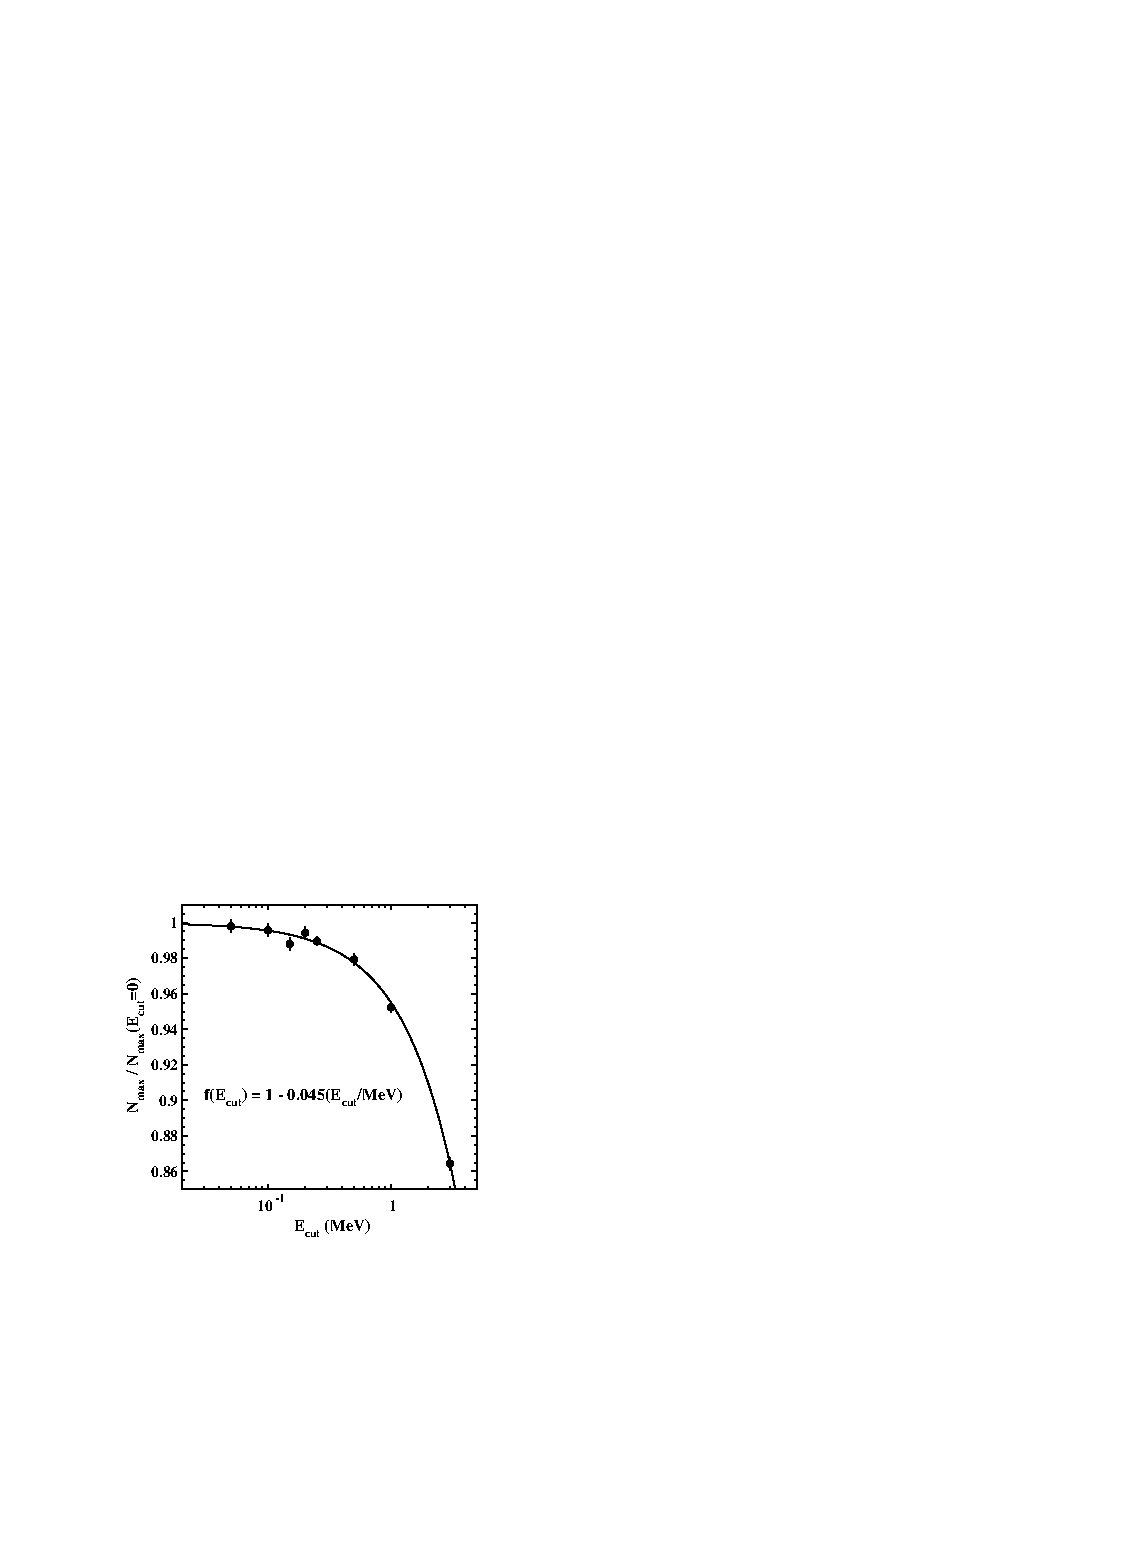
\includegraphics[width=0.8\textwidth]{CorsikaCutoff}
    \caption{The dependence of $N_\text{ch}(E > E_\text{cut})$ on $E_\text{cut}$, taken from Nerling \cite{nerling2006electron}. Note the relatively small fractional change from zero to \SI{1}{MeV}.}
\end{figure}

\section{Ray Tracing}

\subsection{Random Ray Generation} \label{sec:generation}

Once the number of observed photons is known, each must be ray-traced to the detector. Fluorescence photons are emitted isotropically and travel directly from the shower to the detector. The fraction captured is equal to the fraction of a sphere covered by the detector.
\begin{equation} \label{eq:fluor_frac}
    f_\text{fl} = \frac{r^2}{4d^2} \cos{\theta}
\end{equation}
$\theta$ is the angle between the detector axis and the emission point, $r$ the radius of the stop, and $d$ the distance from the detector to the emission point. This fraction is multiplied by the mirror reflectance, photomultiplier quantum efficiency, and wavelength filter transmittance to convert the number of photons to the number of detected photoelectrons. Physically, these inefficiencies occur within the detector, but it is equivalent to apply them before ray tracing. The user may define a thinning rate, $T = $ \texttt{fluor\_thin}, which reduces the number of unique simulated photons by a factor of $T$. Each of the $N / T$ photons is recorded $T$ times when it reaches the detector. The ray for each detected fluorescence photon is placed at the location of the shower, and randomly shifted up or down within the current step. The starting time of the ray is adjusted accordingly. Each ray is traced to a random point on the stop.

Unlike fluorescence, Cherenkov photons must be reflected from the ground. When determining the fraction seen, it is assumed that most are reflected near the ground impact of the shower core. The Lambertian model of diffuse reflection is used, which assumes that the amount of light captured scales like the apparent size of the surface. Defining $f_\text{cv}$ as the Cherenkov fraction, we write $f_\text{cv} = A \cos{\phi} \text{d} \Omega$, where $\phi$ is the angle of the observer with respect to the ground's normal vector. Integrating this over a half sphere gives the normalization factor $A = 1 / \pi$. Let $f_s$ be the fraction of a sphere covered by the detector relative to the ground reflectance point, with the same form as Equation \ref{eq:fluor_frac}. Assuming $f_s$ is small, we can write $\text{d}\Omega = 4 \pi f_s$. Therefore,
\begin{equation}
    f_\text{cv} = 4 \cos{\phi} f_s.
\end{equation}
The detector efficiency and computational thinning are applied as they were for fluorescence. The angle between Cherenkov photons and the shower axis obeys the following distribution given by Stratton \cite{stratton2012ta}:
\begin{equation} \label{eq:ckv_angle}
\begin{gathered}
    A(\theta) = e^{-\theta / \theta_c} \\
    \theta_c = 0.83 E_\text{thr}^{-0.67}.
\end{gathered}
\end{equation}
For each simulated Cherenkov photon, a direction is chosen from this distribution, and the position is found via the same shifting method used for fluorescence. These photons are propagated until they collide with the ground plane, where they are reflected to random locations on the stop.

\subsection{Detector Optics} \label{sec:optics}

After reaching the stop, both fluorescence and Cherenkov photons must be traced through the detector optics. This involves refraction by the Schmidt corrector. The shape of the corrector is given by Malacara \cite{malacara2004optics}.
\begin{equation}
    Z(S) = \frac{S^2}{4(n - 1)r_m^3}(S^2 - S_\text{max}^2)
\end{equation}
$S$ is the distance from the axis, $n$ the lens' index of refraction, $r_m$ mirror's radius of curvature, and $S_\text{max}$ the radius of the stop. As explained in Section \ref{sec:intro_recon}, the quadratic term and inner portion of the corrector are removed. A local minimum of $Z(S)$ occurs at $S_\text{max} / \sqrt{2}$, and is set as the inner boundary of the corrector.
\begin{equation}
Z(S)=
    \begin{cases}
    \frac{S^4}{4(n - 1)r_m^3} & \text{ if } S > S_\text{max} / \sqrt{2} \\
    0 & \text{ if } S \leq S_\text{max} / \sqrt{2}
    \end{cases}
\end{equation}
Performing the refraction requires finding lens normal $\vec{n}_l$ for any $(x, y)$ on the stop. If $S \leq S_\text{max} / \sqrt{2}$, the normal is $(0, 0, 1)$. If $S > S_\text{max} / \sqrt{2}$, then the x and y components must point back toward the z-axis, so they are set to $-x$ and $-y$. The ratio of the z component to the planar component is $1 / Z'(S)$, which is guaranteed to be non-infinite for $S > S_\text{max} / \sqrt{2}$. Therefore, the normal vector is
\begin{equation}
\begin{aligned}
\vec{n}_l &= \left(\frac{S}{Z'(S)}, -x, -y\right) \\
          &= \left(\frac{(n - 1)r_m^3}{S^2}, -x, -y\right).
\end{aligned}
\end{equation}
This can be normalized to obtain $\hat{n}_l$, the unit normal vector. If the incident ray is not parallel to $\hat{n}_l$ and has direction $\vec{d}$, then the axis of rotation for the refraction is $\hat{n}_l \times \vec{d}$. The angle of rotation about this axis is determined by Snell's law. When refracting across the flat back surface of the corrector, the same procedure is used, but with a normal vector of $(0, 0, -1)$ and a check for total internal reflection. The two refractions are performed back-to-back, without accounting for the finite corrector thickness.

Rays are then traced to their intersection with the spherical mirror. The sphere is centered at the origin and defined by $x^2 + y^2 + z^2 = r_m^2$. Given the ray's starting position $(x_0, y_0, z_0)$ and velocity $(v_x, v_y, v_z)$, the times when the ray will cross the sphere can be found by solving
\begin{equation}
    (x_0 + v_x t)^2 + (y_0 + v_y t)^2 + (z_0 + v_z t)^2 = r_m^2.
\end{equation}
If there are two roots, then the one giving a more negative z-value is chosen. If there are no roots or the intersection points lie outside the edge of the mirror (which is only a section of the sphere), the ray is thrown out. Valid rays are traced to their reflection points, checking for collision with the back of the focal surface. Reflection subtracts $2 \vec{v} \cdot \hat{n}_m$ from the velocity, where $\hat{n}_m$ is the mirror normal at the reflection point. Because the center of curvature is the origin, $\hat{n}_m$ is simply the negative unit position of the reflection point.

Rays are traced to the spherical detection surface with the same method used for the mirror. Any photons outside the boundaries of the pixel array are thrown out. If the position of the focal impact point is $\vec{f}$, then the pixel bins $b_x$ and $b_y$ can be found using the following:
\begin{gather}
    \begin{gathered}
        \theta = \arctan{\frac{f_y}{f_z}} \\
        \phi = \arctan{\frac{f_x}{f_z}}
    \end{gathered} \qquad
    \begin{gathered}
        b_y = \left\lfloor \frac{\theta}{\Delta \alpha} \right\rfloor + n \\
        b_x = \left\lfloor \frac{\phi}{\alpha \cos{\theta}} \right\rfloor + n
    \end{gathered}
\end{gather}
$2n$ is the diameter of the array in pixels, and $\Delta \alpha$ is the angular size of each pixel. $b_t$ is determined with a straightforward temporal binning. Certain reasonable limits are placed on the minimum and maximum allowed times so the underlying data structure can be given a finite size. If the time is within these bounds, the counter at the $(b_x, b_y, b_t)$ bin is incremented by the thinning level.

\section{Addition and Filtering of Noise} \label{sec:noise}

Night sky background noise obeys a Poisson distribution.
\begin{equation} \label{eq:poisson}
    P(k: \lambda) = e^{-\lambda}\frac{\lambda^k}{k!}
\end{equation}
$\lambda$ is the mean rate and $k$ is a particular number of noise photons. Noise is added by iterating through each $(b_x, b_y, b_t)$ bin and randomly sampling from the Poisson distribution, where
\begin{equation}
    \lambda = \Omega_p  A_s  T_b  \mu.
\end{equation}
$A_s$ is the area of the stop, $T_b$ the time per bin, and $\Omega_p$ the solid angle of a single pixel. $\mu = \SI{4.9e5}{sr^{-1}.cm^{-2}.s^{-1}}$ is the night sky noise level. This value is based on Telescope Array observations of 6 photoelectrons per \SI{100}{ns} per square degree per \SI{4}{m^2}. Noise from pixels pointing toward the ground also obeys a Poisson distribution, but the mean is lowered by a factor of ten. Most noise filtration steps involve comparing signal values to thresholds, which are computed as multiples of $\sigma$. For a Poisson distribution, $\sigma=\sqrt{\lambda}$. However, a direct application of this formula tends to give more lenient thresholds than would be found with the same multiple of $\sigma$ on a Gaussian. To solve this problem, an upper bound is chosen for the Poisson threshold probability. For a $3\sigma$ threshold, the $3\sigma$ tail of a Gaussian is integrated to give probability \num{0.0014}. To match this, the Poisson threshold is increased until the above-threshold probability is less than \num{0.0014}.

Noise filtration begins with the uniform subtraction of $\lambda$ from each bin. Triggering logic is then applied to omit frames and showers where no significant signal is seen. In each time frame, the largest cluster of signals above $6\sigma$ is found. If this cluster contains more than five pixels, the frame is triggered. If no frames are triggered, then a reconstruction is not attempted. Otherwise, a set of anchor points is chosen, starting with any bins above $6\sigma$ which are in a triggered frame. A shower-detector plane is fit to the anchor points (see Section \ref{sec:recon}). Any anchor points more than some angle $\theta_\text{max}$ from the plane are removed, according to
\begin{equation}
    \arcsin(\hat{n}_p \cdot \hat{v_i}) > \theta_\text{max}.
\end{equation}
$\hat{n}_p$ is the plane normal vector, and $\hat{v_i}$ the pointing direction of a particular pixel. The remaining anchors are used as the starting points of a breadth-first traversal of the 3D histogram. The traversal bleeds outward from anchor points through any $3\sigma$ bins which occupy the eight spatially adjacent or two temporally adjacent spaces. All anchor points and accessible $3\sigma$ points are considered non-noise; everything else is removed.

\section{Reconstruction} \label{sec:recon}

If a pixel has direction $\hat{v_i}$, and the shower-detector plane has normal vector $\hat{n}_p$, then the deviation of that pixel from the plane can be measured by $(\hat{v_i} \cdot \hat{n}_p)^2$. This gives the following $\chi^2$ for the shower-detector plane, taken with modification from Stratton:
\begin{equation}
    \chi^2 = \sum_i  N_i \cdot (\hat{\nu_i} \cdot \hat{n})^2.
\end{equation}
$N_i$ is the total number of non-noise photoelectrons observed by the pixel \cite{stratton2012ta}. Stratton performs the summation only over ``good tubes.'' The choice of good tubes depends partially on the choice of the shower-detector plane, so the fit must be performed iteratively. Our good tubes have already been determined using the noise filtration methods from the previous section, eliminating the need for an iterative minimization. The minimum of the chi square can be found analytically by taking $\hat{n}_p$ to be the eigenvector of a symmetric matrix $M$ with the smallest eigenvalue, where
\begin{equation}
    M_{jk} = \sum_i  N_i \nu_{ij} \nu_{jk}.
\end{equation}

The monocular fit uses the analytic time profile of Equation \ref{eq:time_prof}. Each pixel's $\chi_i$ is found by rotating its direction to the shower-detector frame and taking the angle with the x-axis. $t_i$ is the mean of the photon arrival times. Due to the binned nature of the data, a Sheppard correction of $T_b^2 / 12$ is added to the variance of the mean. $R_p$, $\psi$, and $t_0$ can be found by fitting Equation \ref{eq:time_prof} against the $(\chi_i, t_i)$ points. Once this monocular fit has been performed, a decision is made whether to perform the Cherenkov fit. The monocular $R_p$ and $\psi$ can be used to estimate the ground impact point of the shower. If the impact point is visible by the detector and at least some angle $\theta_\text{min}$ from the edge of the field of view, a search is performed over all below-horizon pixels and the brightest pixel is found. If the brightest pixel has a signal above $6\sigma$, it is selected as the reflectance point and its direction is extended to the ground. The Cherenkov reconstruction is then performed similarly to the monocular reconstruction, with the only difference being the replacement of $R_p$ with $d \sin(\psi + \alpha)$ (see Equation \ref{eq:ckv_relation}).}
\newcommand{\results}{
    \chapter{RESULTS}
    \thispagestyle{fancy}
    \section{Case Study}

A single test case was simulated to visually determine the brightness of the Cherenkov peak and any interesting features. The test shower had an energy of \SI{e19}{eV}, an impact parameter of \SI{10}{km}, and an axis pointing slightly rightward and away from the detector. Figure \ref{fig:typical_map} shows the view from the detector after the addition of noise. The sky-ground boundary is visible as a drop in the level of background noise at $y = 120$. Figure \ref{fig:typical_graph} shows the time profile before the addition of noise. In the first portion, the shower moves downward and produces fluorescence photons. At about \SI{0.128e-3}{s}, there is a sharp peak from the reflected Cherenkov radiation. The tails of this peak are caused by Cherenkov rays with large deviations from the shower axis. The brightness of the Cherenkov peak prompts a hybrid reconstruction. Before reconstruction, noise filtration is performed. For a well-behaved shower like this, the core of the fluorescence track remains intact, and only 1-2 photoelectron signals near the fringes are removed. Figure \ref{fig:typical_denoise_map} shows the spatial profile after this process. The actual impact parameter and angle are \SI{10}{km} and \ang{72.5}. The monocular reconstruction gives \SI{9.75}{km} and \ang{71.3}, whereas the Cherenkov reconstruction gives \SI{10.6}{km} and \ang{75.2}.

\begin{figure}[!ht]
    \label{fig:typical_map}
    \centering
    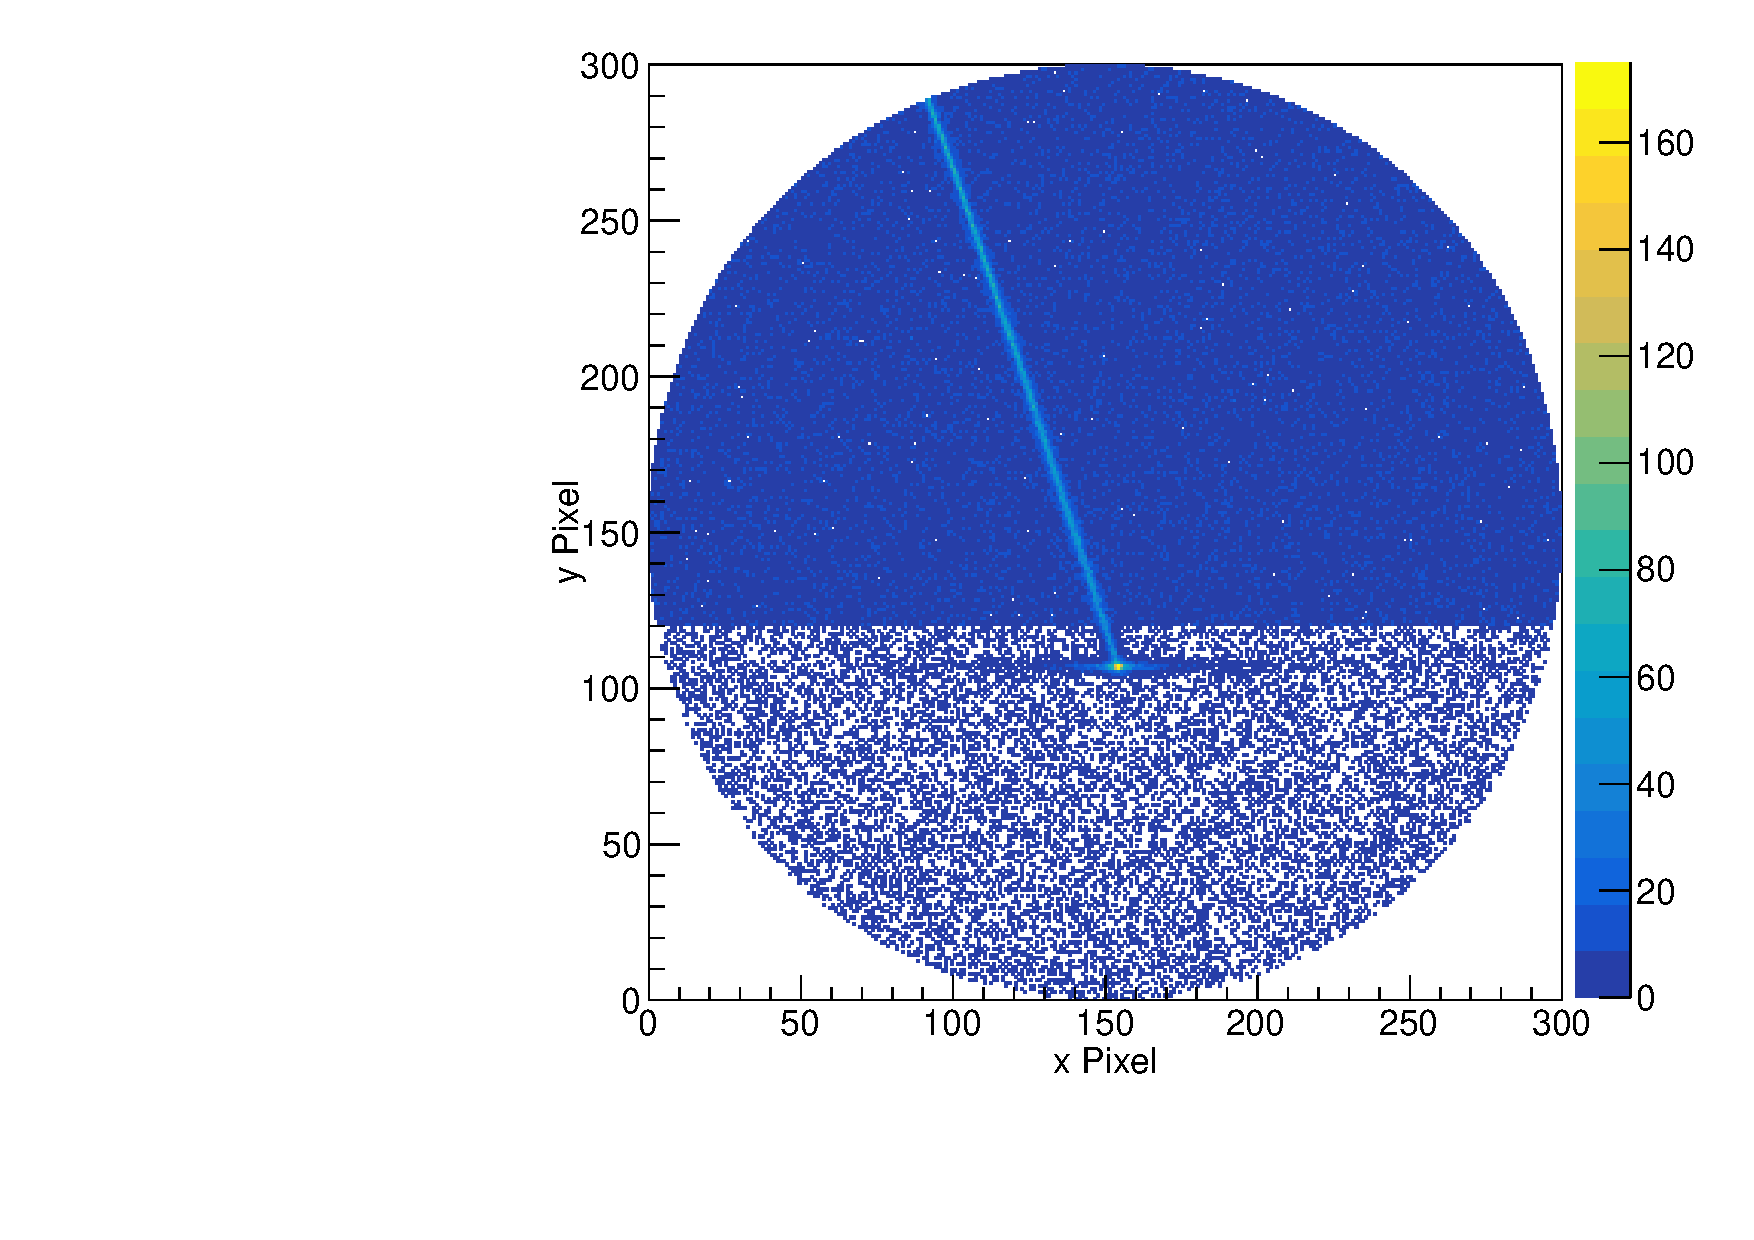
\includegraphics[width=\textwidth]{TypicalShowerMap}
    \caption{A spatial view of a typical shower track with noise added. This event has energy \SI{e19}{eV}, angle \ang{72.5}, and impact parameter \SI{10}{km}.  The ground impact is visible near pixel (150, 100).}
\end{figure}

\begin{figure}[!ht]
    \label{fig:typical_graph}
    \centering
    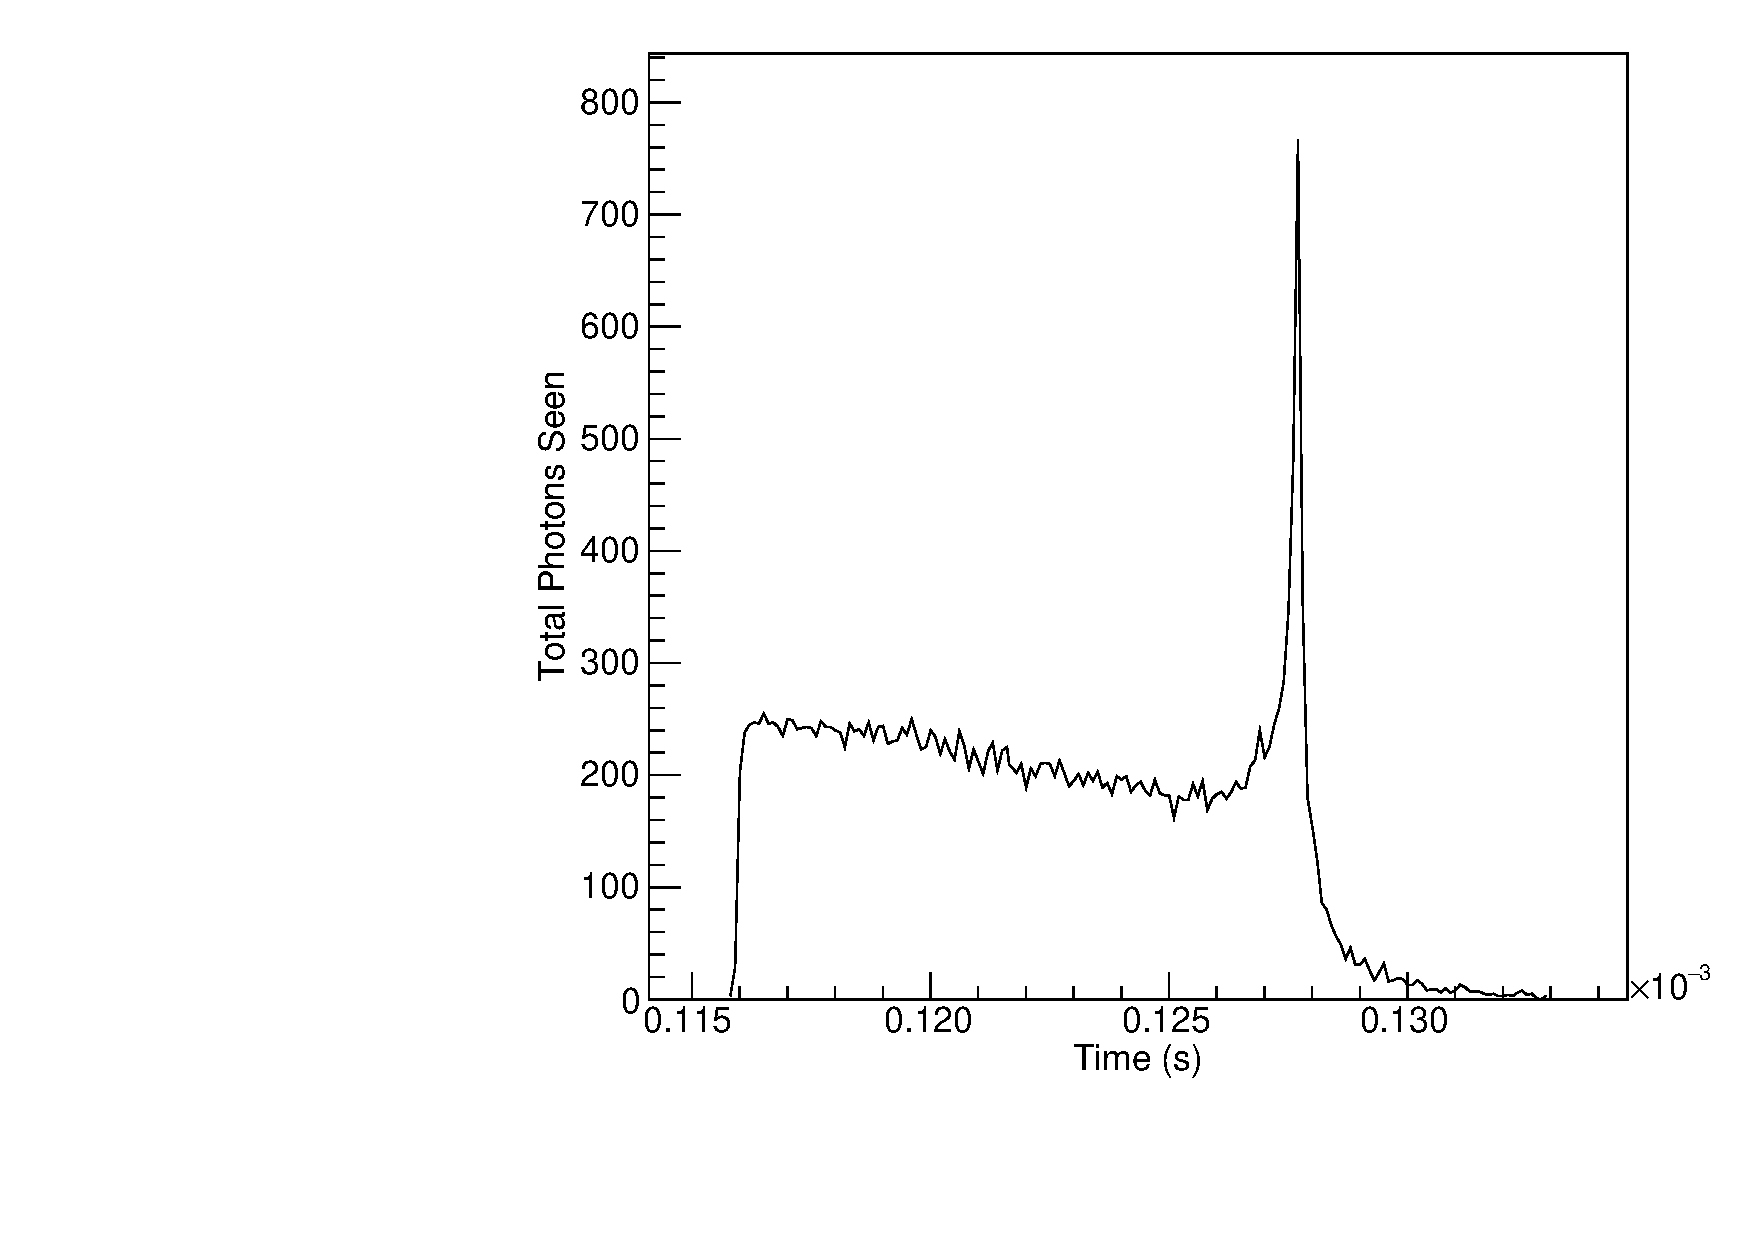
\includegraphics[width=\textwidth]{TypicalShowerGraph}
    \caption{Signal versus time for the event shown in Figure \ref{fig:typical_map}. The Cherenkov peak is visible near \SI{0.128e-3}{s}. The fluorescence portion decays because of the shower direction and because the Gaisser-Hillas maximum has been passed.}
\end{figure}

\begin{figure}[!ht]
    \label{fig:typical_denoise_map}
    \centering
    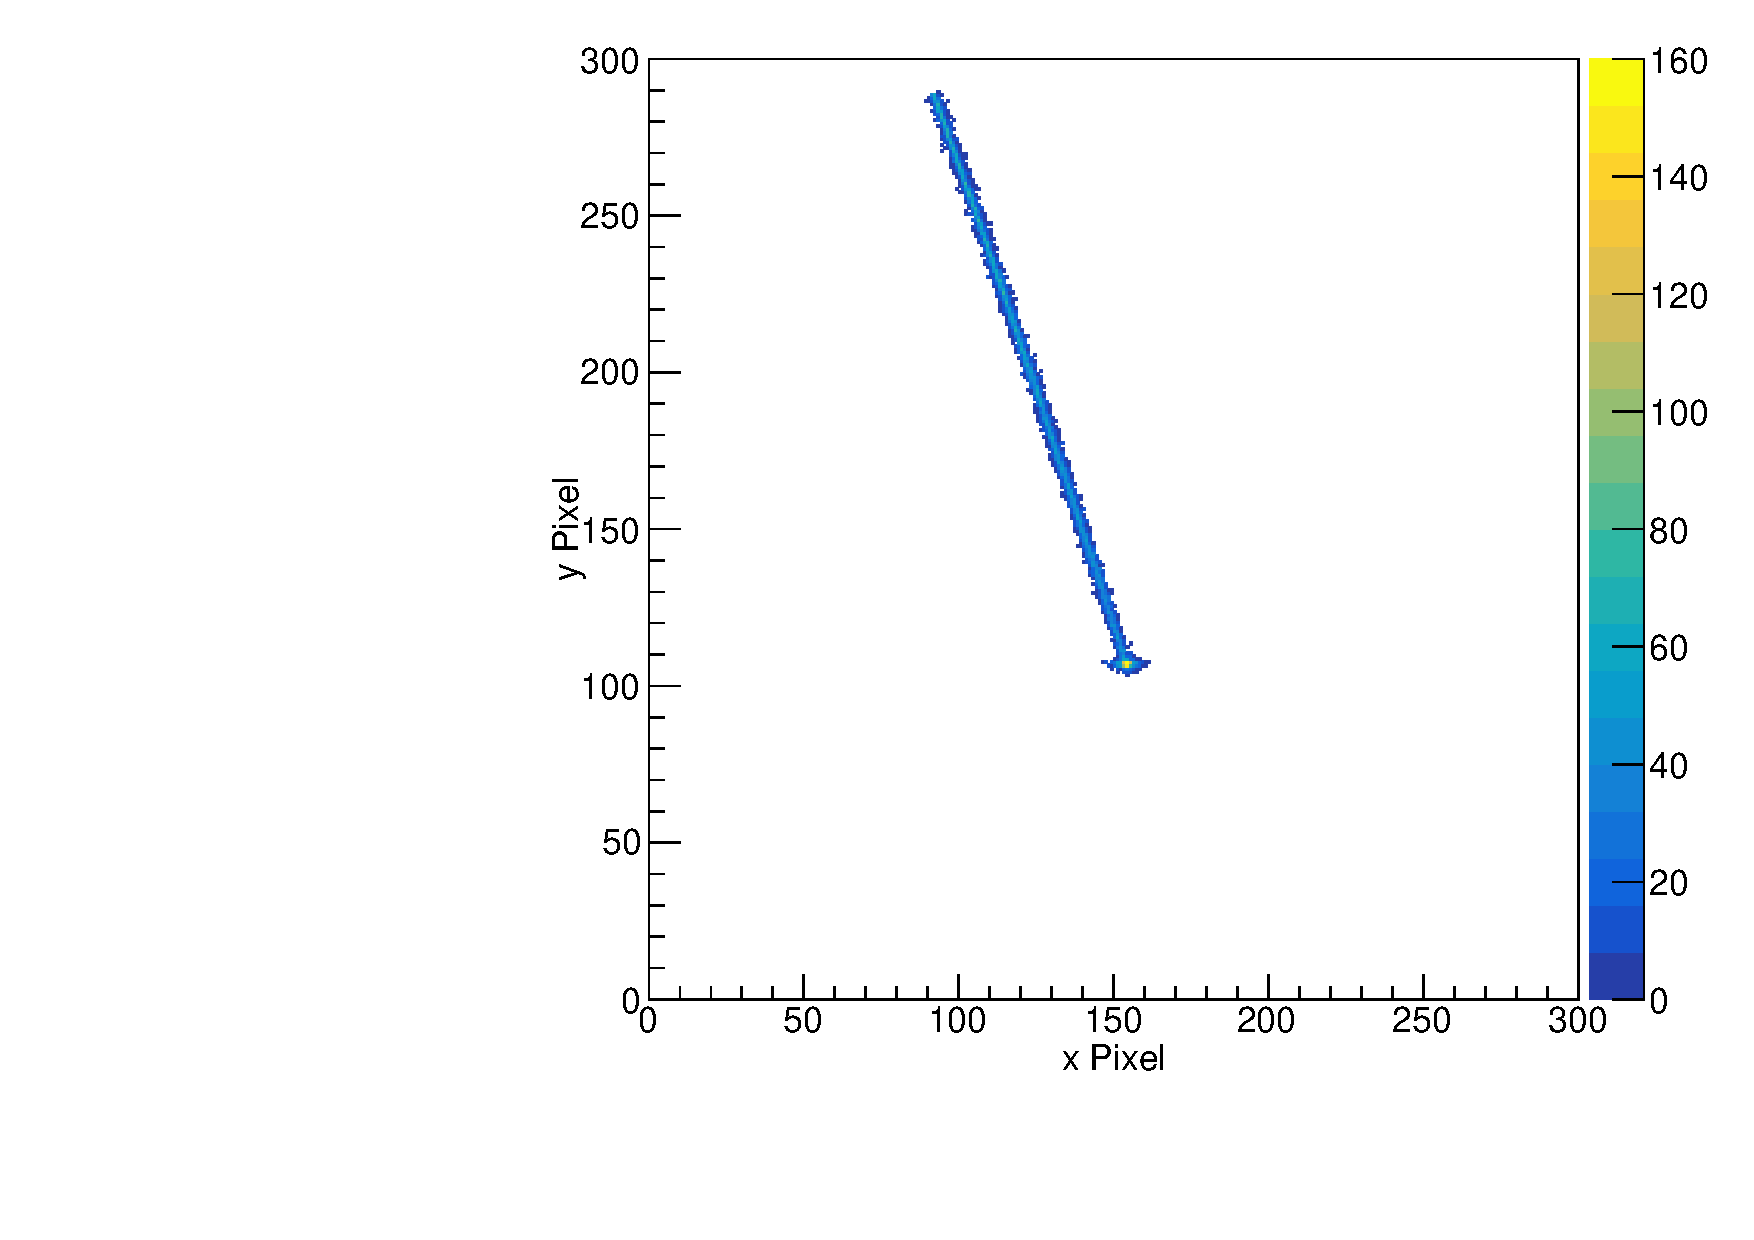
\includegraphics[width=\textwidth]{TypicalDenoiseMap}
    \caption{The shower track from Figure \ref{fig:typical_map} after the removal of noise. The fluorescence core and impact point are still visible, but their fringes have contracted.}
\end{figure}

\section{Monte Carlo} \label{sec:mc_results}

The initial Monte Carlo run simulated \num{12000} triggered showers with a \SI{200}{m} high detector. Impact parameters were distributed between \num{3} and \SI{40}{km}, and energies were chosen from an $E^{-1}$ distribution between \num{e17} and \SI{e21}{eV}. About \num{8300} of the \num{12000} showers met the requirements for Cherenkov reconstruction. In analyzing these events, we examine both error in the impact parameter and error in the angle. However, as Figure \ref{fig:correlation} shows, there is a strong correlation between the two. Because of this, only trends in impact parameter error were examined.

\begin{figure}[p]
    \label{fig:correlation}
    \centering
    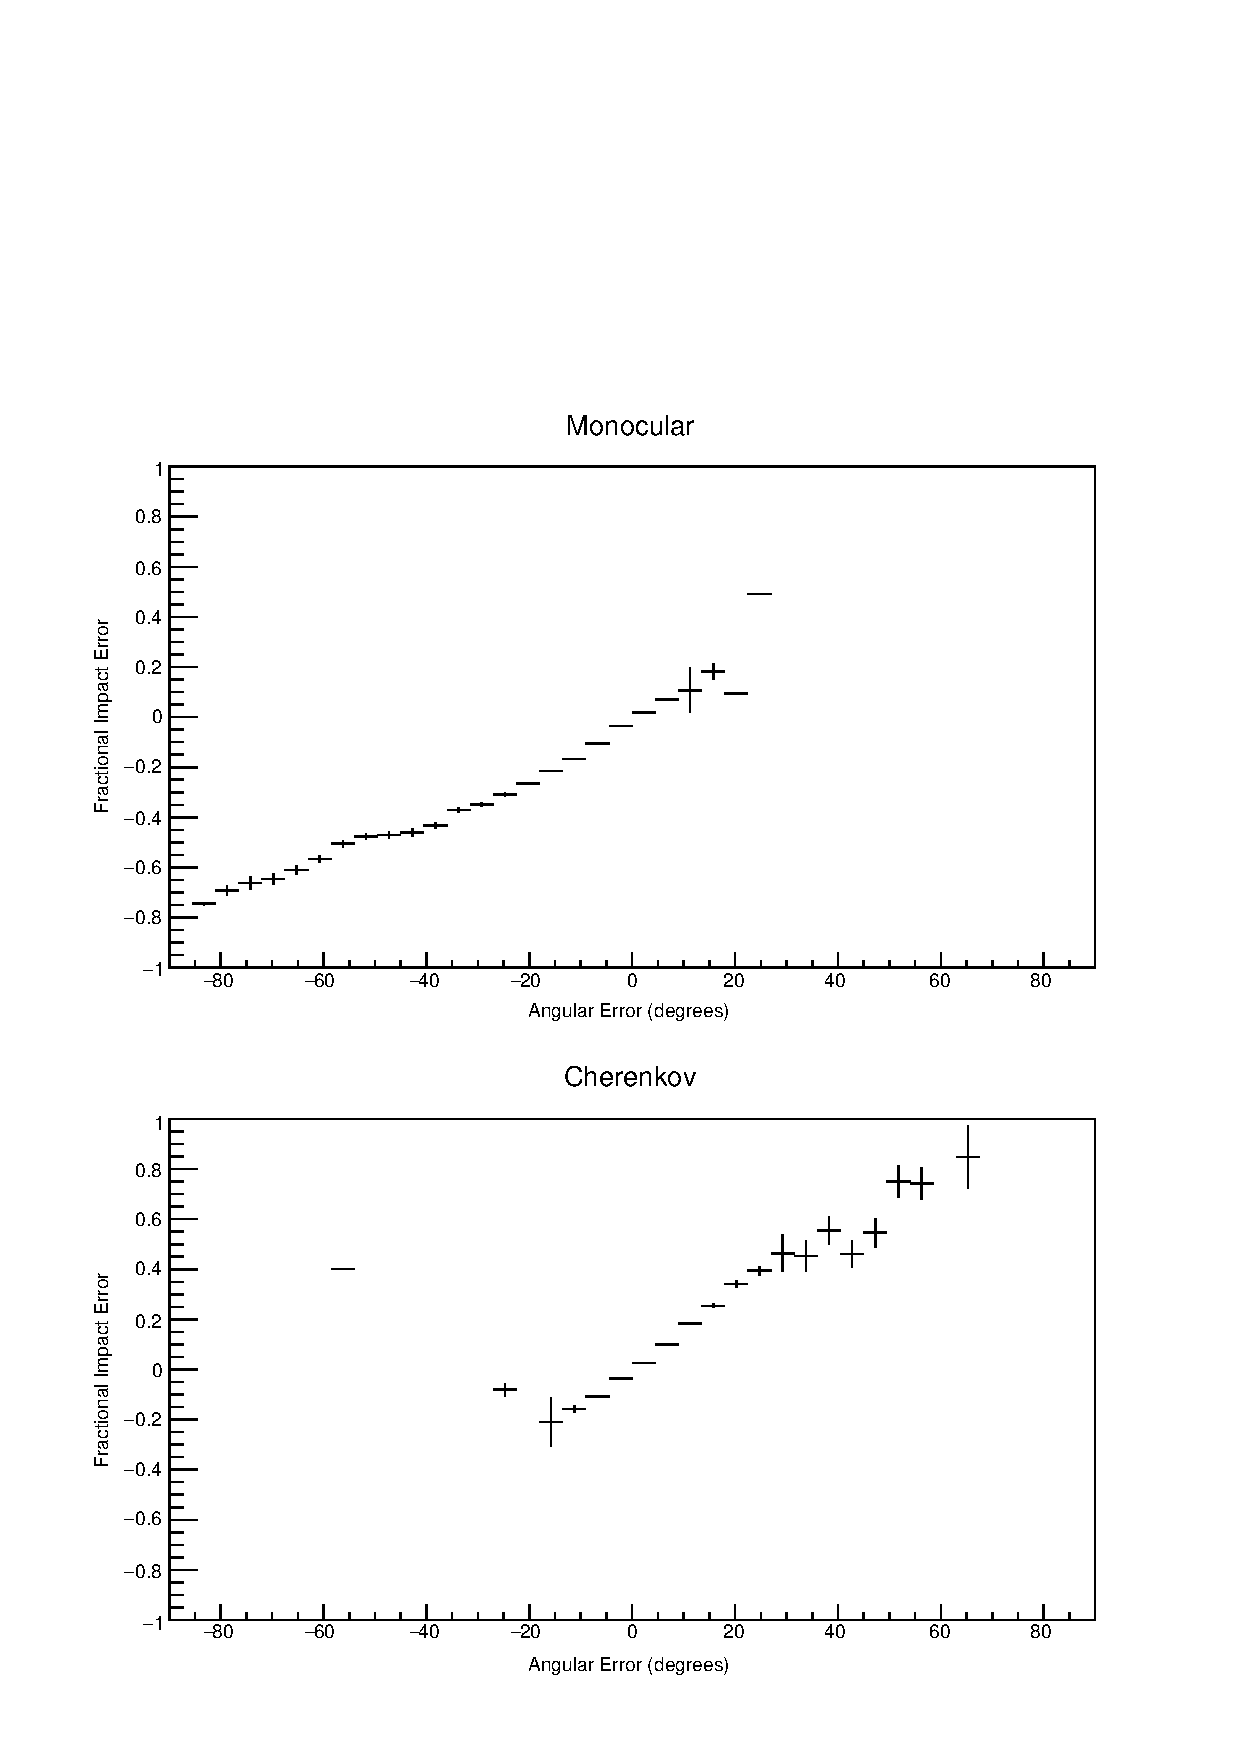
\includegraphics[width=\textwidth]{Correlation}
    \caption{The correlation between error in impact parameter and error in angle, eliminating the need for an independent analysis of each.}
\end{figure}

Figures \ref{fig:error_vs_impact} and \ref{fig:error_vs_angle} illustrate the relationships between fractional impact parameter error and both angle and impact parameter. The Cherenkov reconstruction does well when the impact parameter is less than \SI{25}{km}, although the monocular reconstruction also does fairly well in this range. As expected, the monocular reconstruction does poorly when the shower angle is large. At large angles, the track is compressed in the detector's field of view, and some of the angle versus time information is lost. Somewhat surprisingly, the Cherenkov reconstruction does poorly when the shower angle is small. Below \ang{40}, the average errors exceed the bounds of the graph, and can be on the order of 200-300 percent. These errors are rooted in the relative brightness of the fluorescence track and the Cherenkov reflection point. As the shower angle shrinks, the reflection point gets more distant. While both the fluorescence track and reflection point get dimmer via a standard $1/r^2$ dropoff, the Cherenkov reflection also gets dimmer as $\sin{\alpha}$ due to the nature of Lambertian reflectance ($\alpha$ is the angle of the reflection point from the horizon). This additional $\sin{\alpha}$ factor causes the reflection point to get dimmer more quickly than the fluorescence track. At a certain distance, the reflectance point is overtaken in brightness by the fluorescence track. When this occurs, the ground point algorithm incorrectly chooses a point on the fluorescence track, often adjacent to the horizon. This results in an extreme overestimate of the ground distance and, by extension, of the impact parameter.

\begin{figure}[p]
    \label{fig:error_vs_impact}
    \centering
    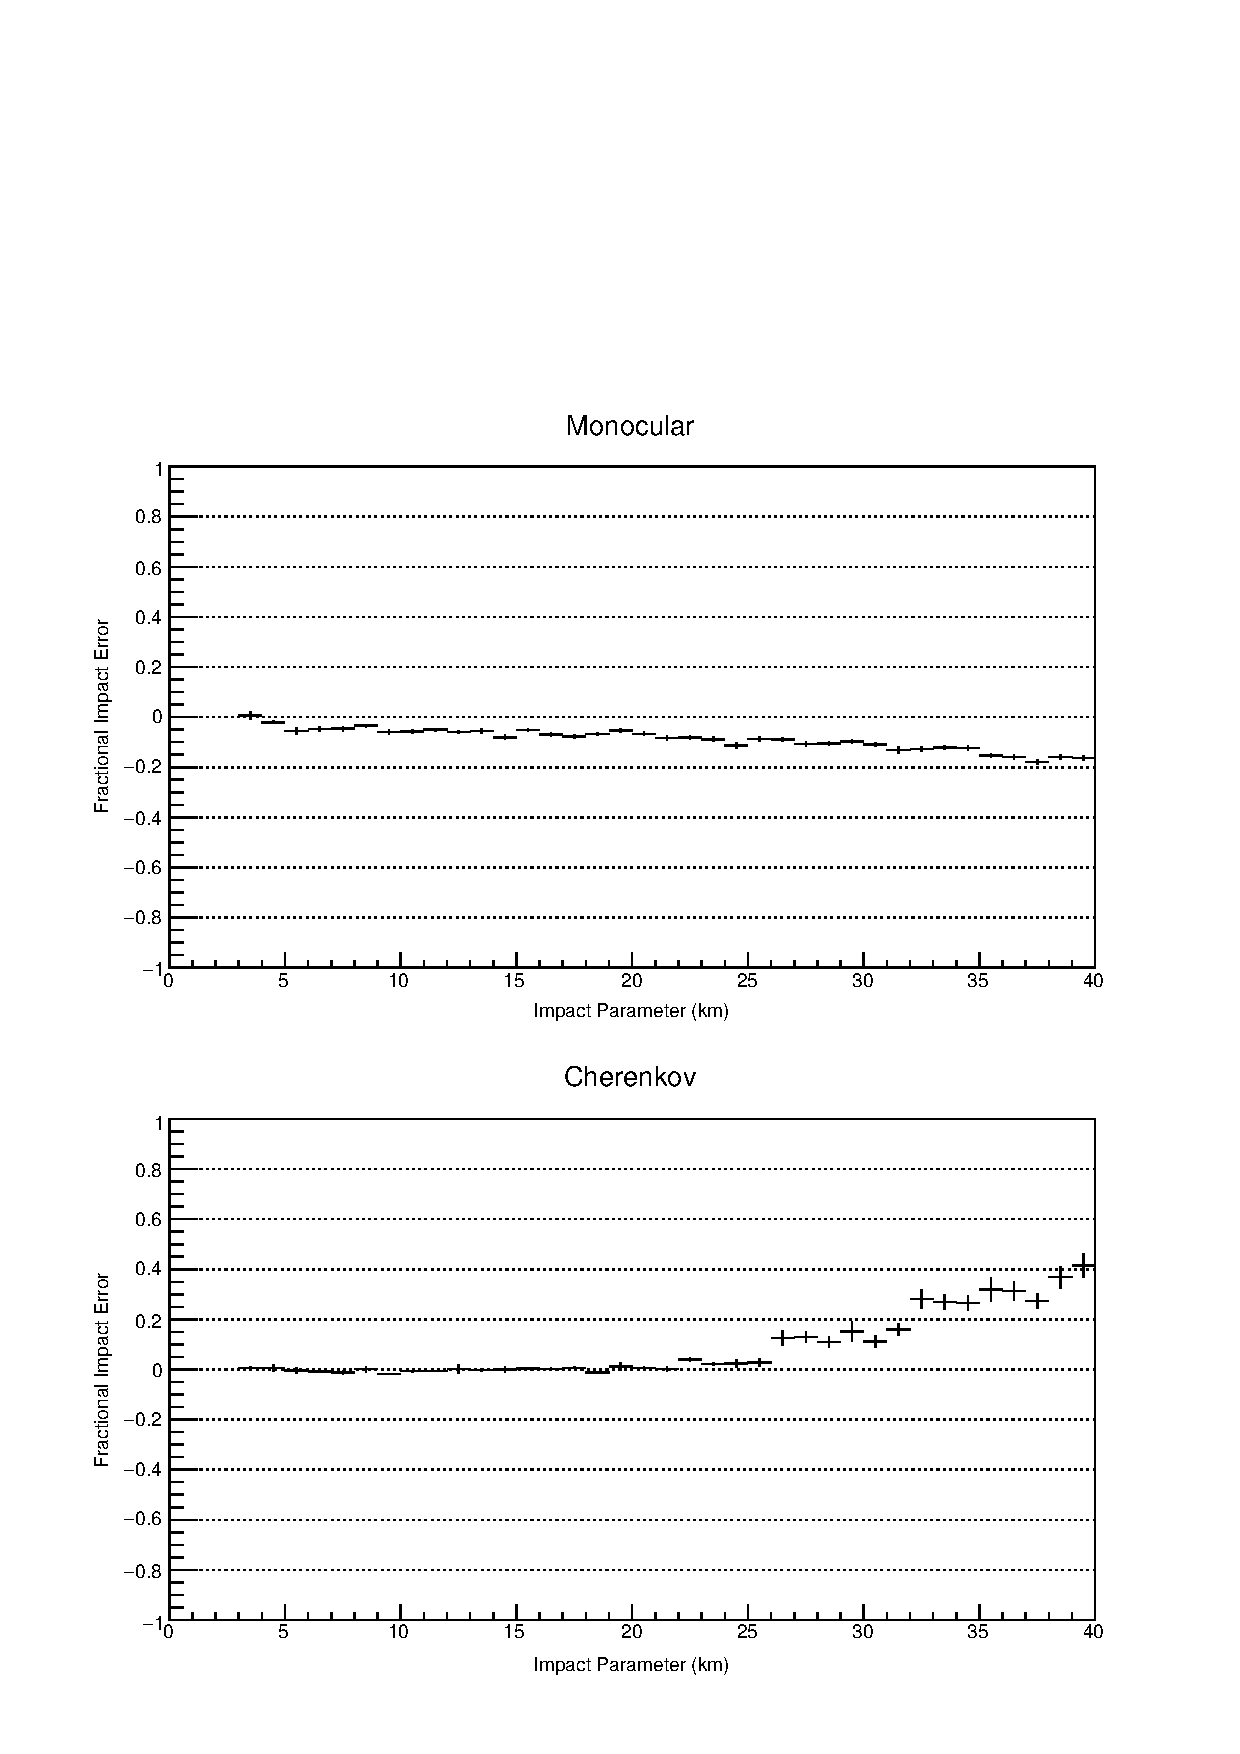
\includegraphics[width=\textwidth]{InitialVersusImpact}
    \caption{Results from the initial run with a \SI{200}{m} high detector. Shows the relationship between reconstruction error and impact parameter, for both monocular and Cherenkov methods.}
\end{figure}

\begin{figure}[p]
    \label{fig:error_vs_angle}
    \centering
    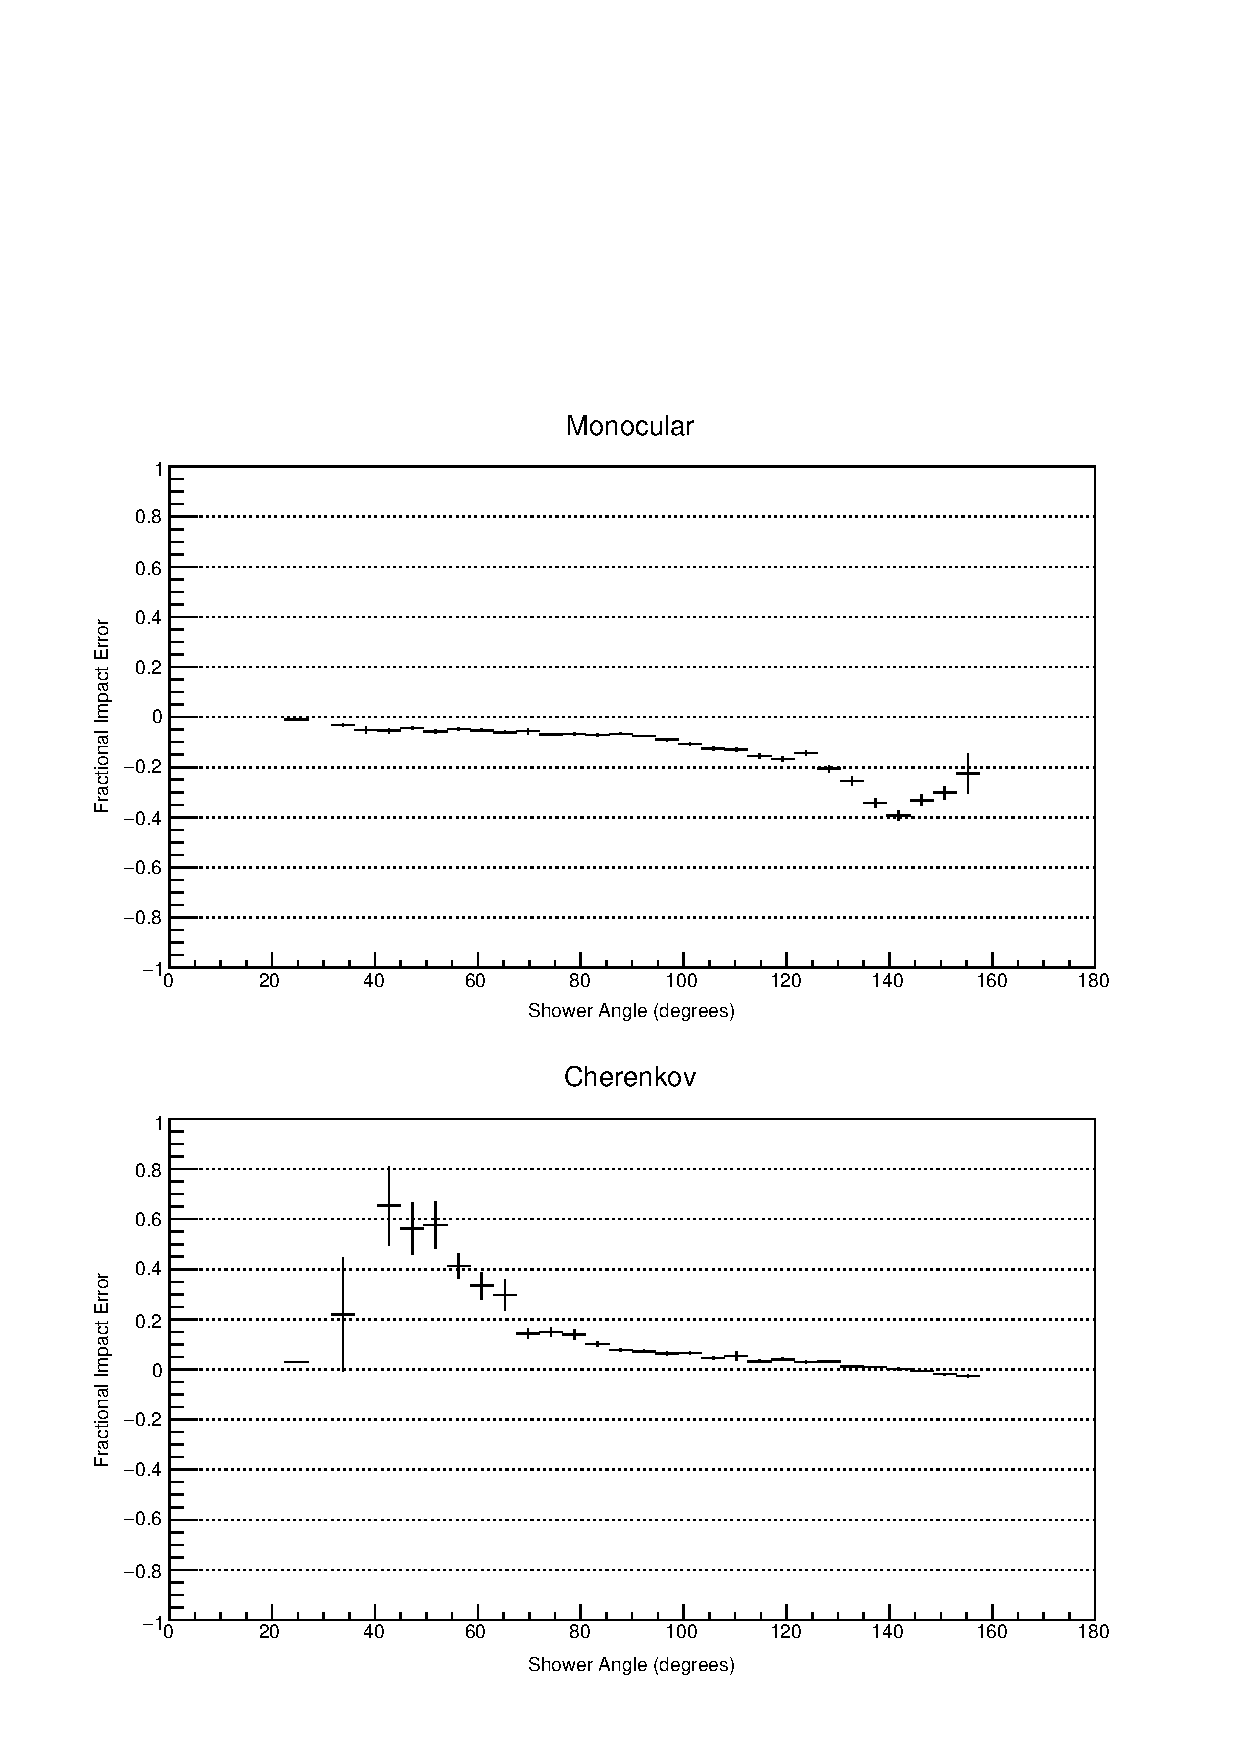
\includegraphics[width=\textwidth]{InitialVersusPsi}
    \caption{Results from the initial run with a \SI{200}{m} high detector. Shows the relationship between reconstruction error and shower angle, for both monocular and Cherenkov methods. Some of the average errors for small angle Cherenkov reconstructions exceed the bounds of the graph.}
\end{figure}

These low-angle failures prompt investigation of the relationship between reconstruction error and ground distance. As shown in Figure \ref{fig:error_vs_gnd}, there is a sharp error increase near \SI{30}{km}. The steepness of the increase indicates that ground distance, like angle, divides the parameter space well. Because the failures are primarily due to dimness of the reflection point and not low resolution (see Section \ref{sec:intro_recon}), the best way to improve the Cherenkov parameter range would be to raise the detector. The second Monte Carlo run does this, increasing the height to \SI{400}{m} and the maximum impact parameter to \SI{60}{km}. \num{4000} triggered showers were simulated, with about \num{2700} allowing Cherenkov reconstruction. The dependence of error on angle was mostly unchanged. Figures \ref{fig:raised_impact} and \ref{fig:raised_gnd} show the new dependence on impact parameter and ground distance. The turnover points increase from about \num{25} and \SI{30}{km} respectively to about \num{40} and \SI{50}{km}. A rough dependence of about $h^{2/3}$ can be conjectured.

\begin{figure}[p]
    \label{fig:error_vs_gnd}
    \centering
    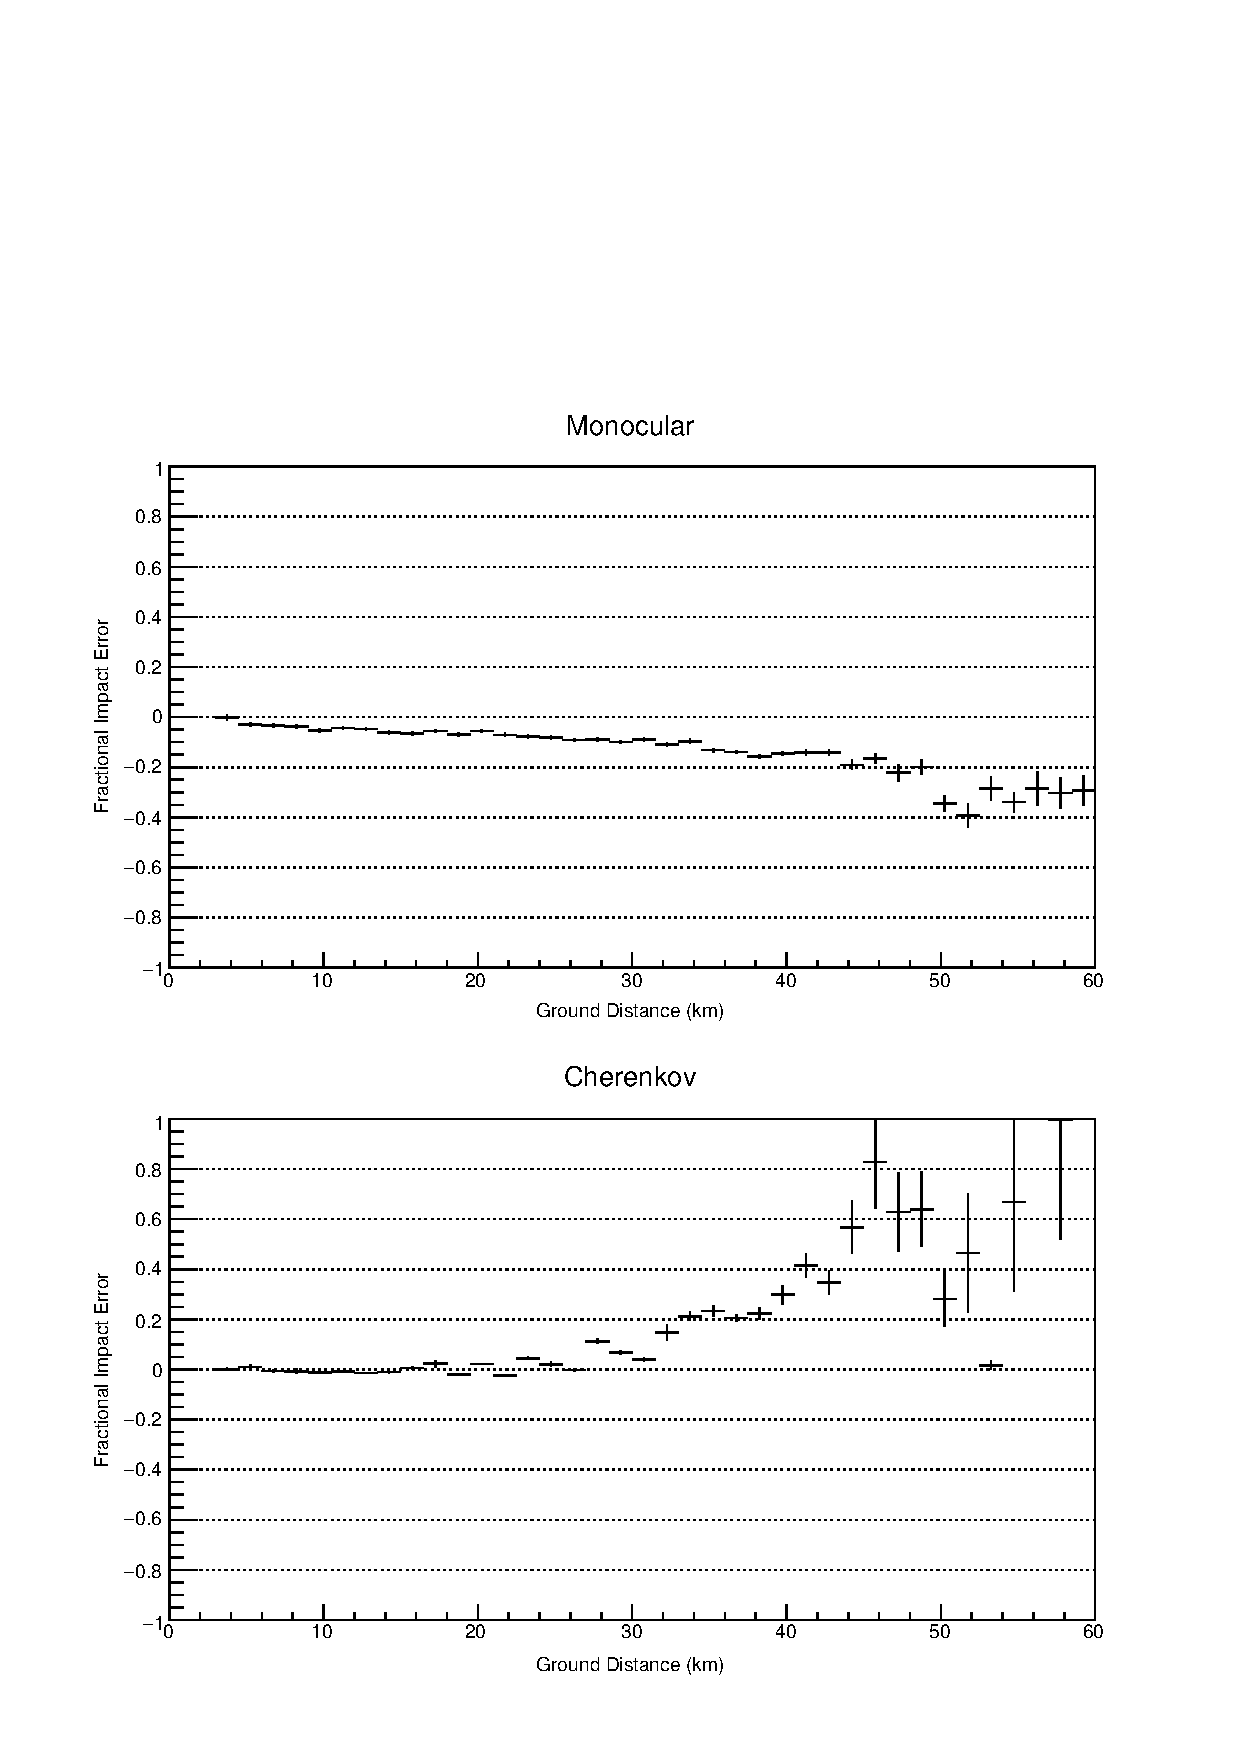
\includegraphics[width=\textwidth]{InitialVersusGround}
    \caption{Results from the initial run with a \SI{200}{m} high detector. Shows the relationship between reconstruction error and ground distance, for both monocular and Cherenkov methods.}
\end{figure}

\begin{figure}[p]
    \label{fig:raised_impact}
    \centering
    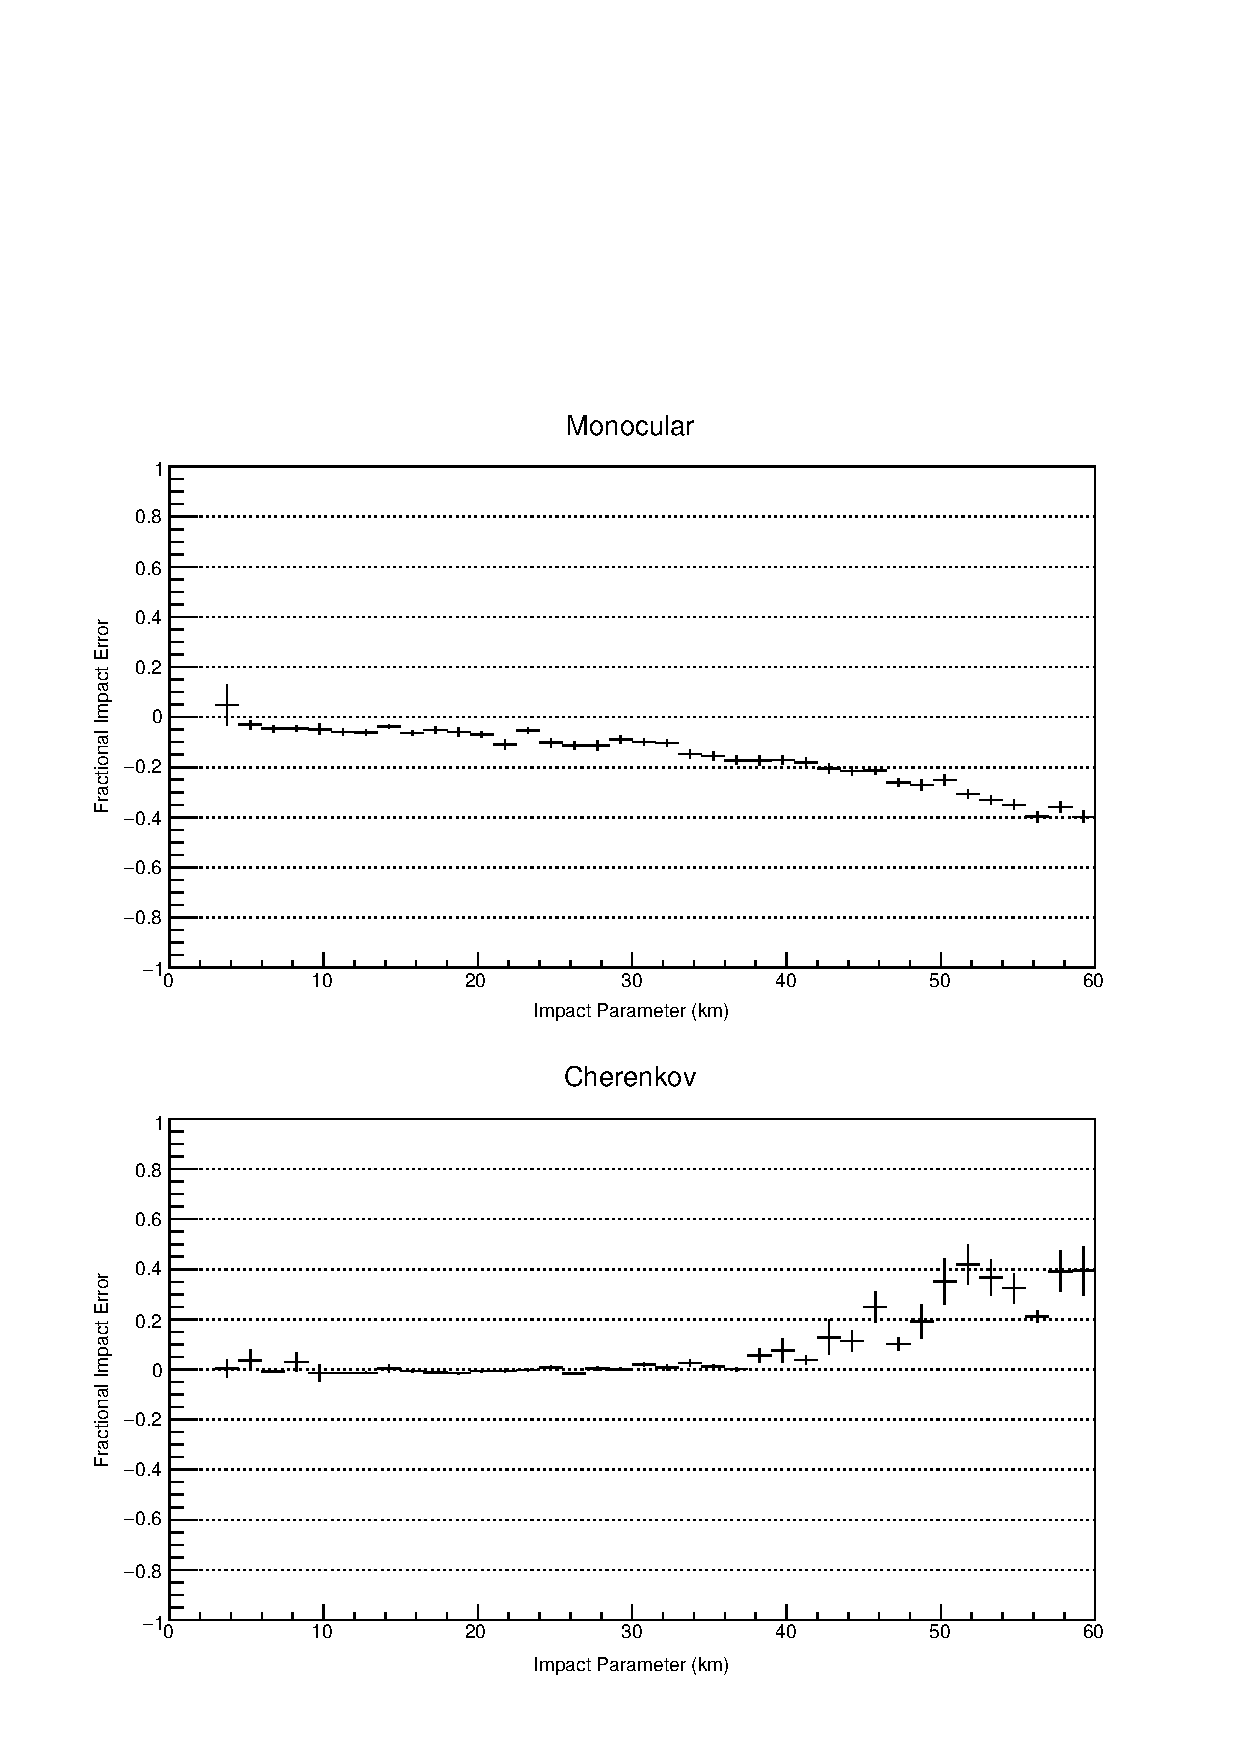
\includegraphics[width=\textwidth]{HighVersusImpact}
    \caption{Results from the second run with a \SI{400}{m} high detector. Shows the relationship between reconstruction error and impact parameter, for both monocular and Cherenkov methods. Note the increased x range of the plot as compared to Figure \ref{fig:error_vs_impact}.}
\end{figure}

\begin{figure}[p]
    \label{fig:raised_gnd}
    \centering
    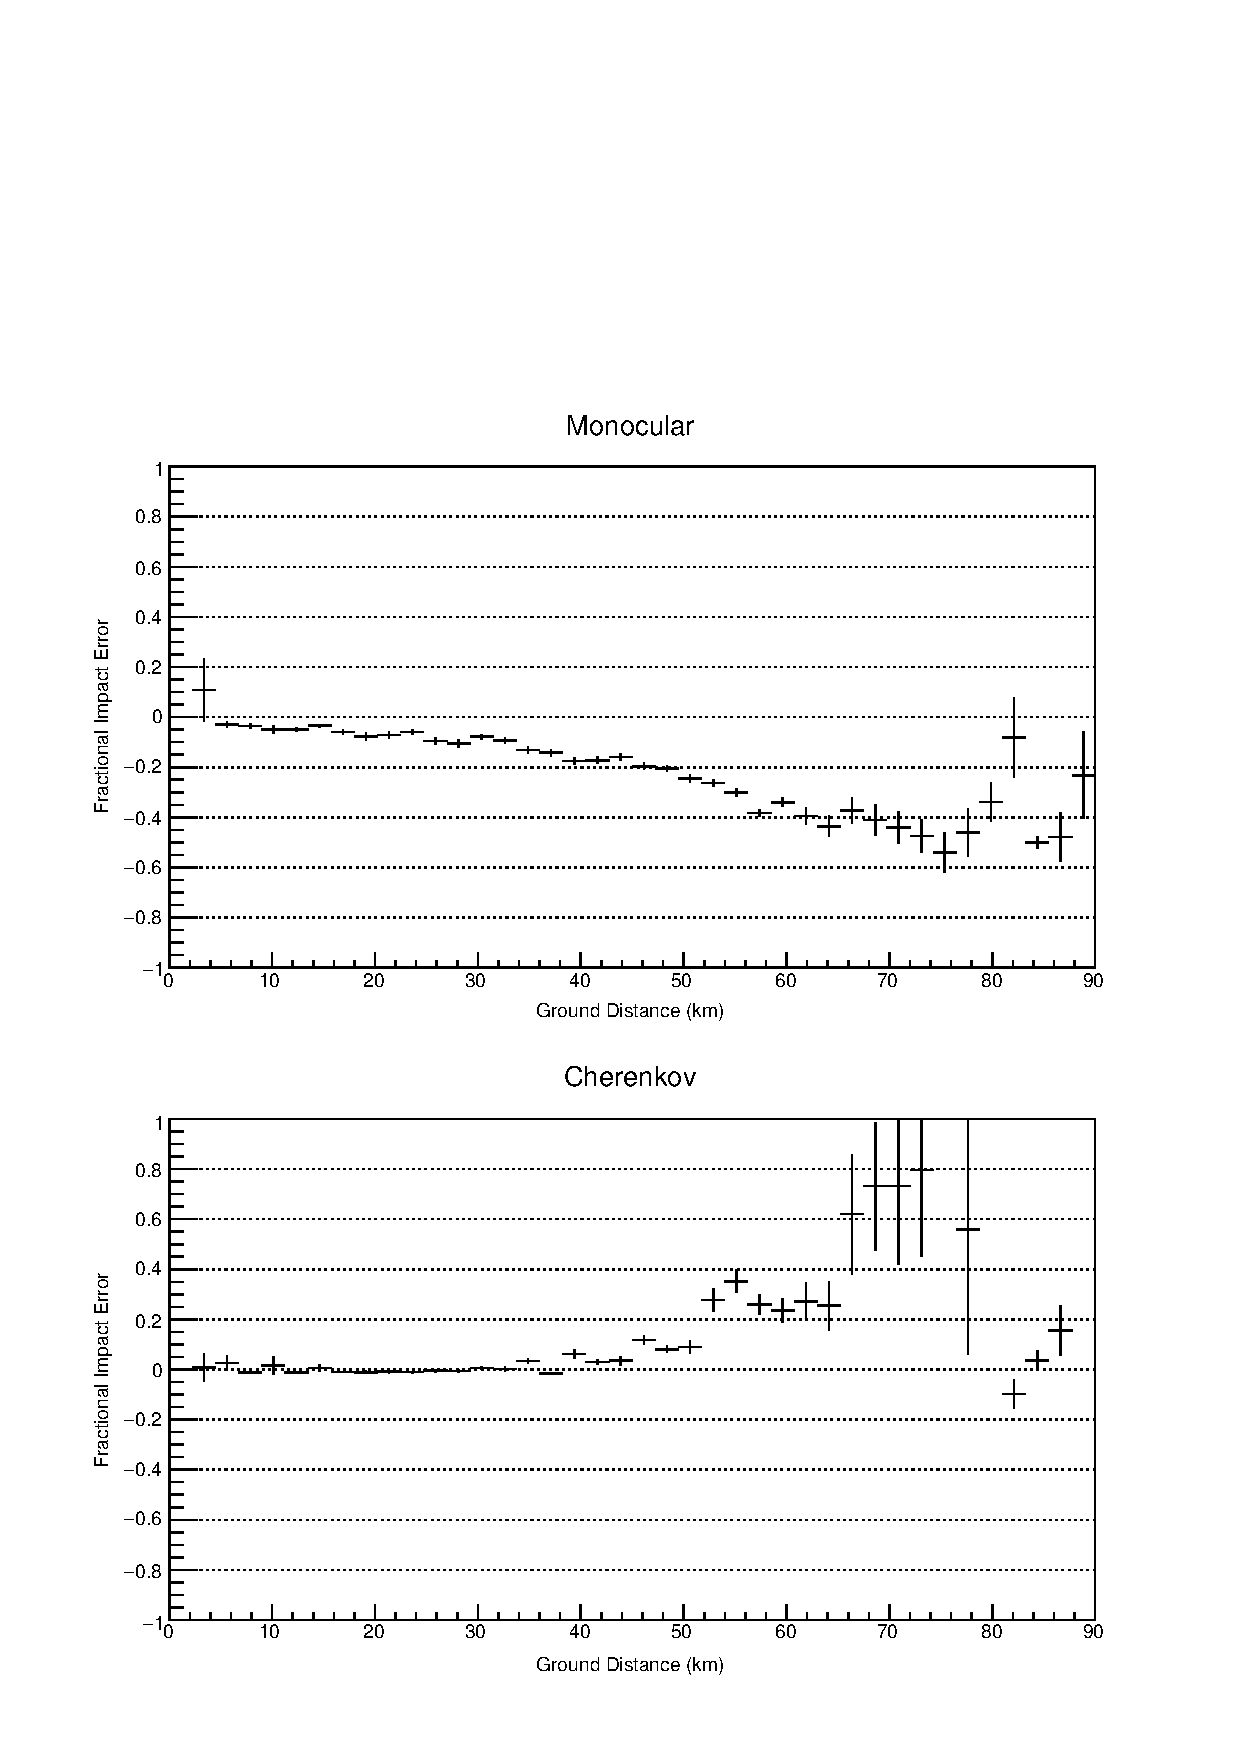
\includegraphics[width=\textwidth]{HighVersusGround}
    \caption{Results from the second run with a \SI{400}{m} high detector. Shows the relationship between reconstruction error and ground distance, for both monocular and Cherenkov methods. Note the increased x range of the plot as compared to Figure \ref{fig:error_vs_gnd}.}
\end{figure}

Based on the results of the \SI{200}{m} simulation, the limits of the Cherenkov reconstruction are set to $\psi > \ang{90}$ or $R_p < \SI{20}{km}$. These bounds are only valid within the subset of the parameter space simulated by the Monte Carlo. Figure \ref{fig:cutoff_hist} compares the overall performance of the two methods under these cuts. Note that there are \num{5573} Cherenkov-reconstructed showers matching the criteria, meaning that the Cherenkov method gives an improvement for about 45 percent of triggered showers. Integrating a Gaussian defined by the parameters in Figure \ref{fig:cutoff_hist} gives an approximation of the expected absolute errors. Under the cuts, the monocular method has an average absolute error of 15.6 percent, while the Cherenkov method has an average absolute error of 10.7 percent. An increase in below-horizon resolution could improve the Cherenkov reconstruction, although it would be unlikely to alter the cuts.

\begin{figure}[p]
    \label{fig:cutoff_hist}
    \centering
    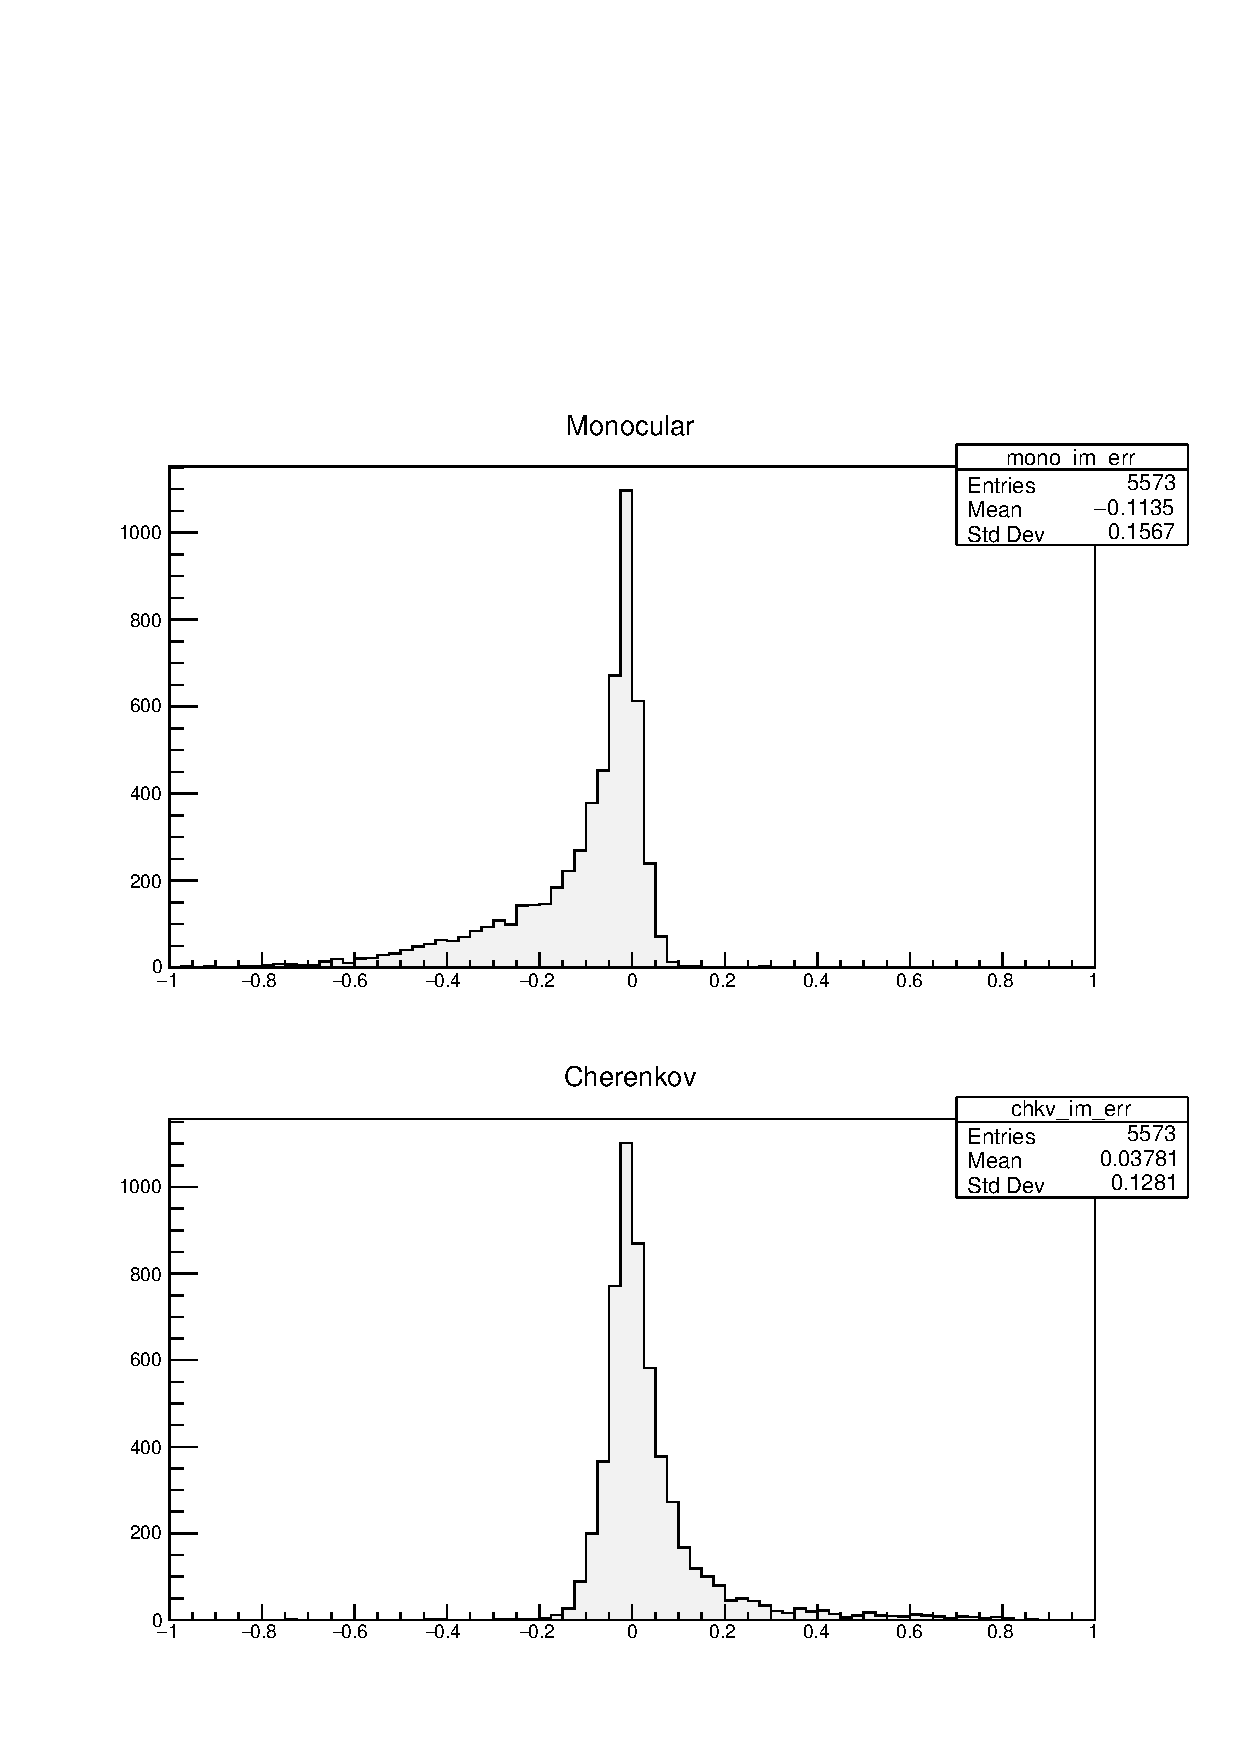
\includegraphics[width=\textwidth]{FinalErrors}
    \caption{The distribution of impact parameter errors from the initial run with a \SI{200}{m} high detector. Cuts of $\psi > \ang{90}$ or $R_p < \SI{20}{km}$ have been applied for the best Cherenkov reconstruction conditions.}
\end{figure}}
\newcommand{\discussion}{
    \chapter{DISCUSSION}
    \thispagestyle{fancy}
    The simulation makes a number of simplifying assumptions, one of which is a lack of atmospheric scattering. Stratton describes the two main mechanisms, Rayleigh and aerosol scattering \cite{stratton2012ta}. Both give some attenuation between the shower and the detector. Assuming this attenuation affects fluorescence and scattered Cherenkov equally, while the number of detected photons would tend to be lower, the relative heights of the fluorescence and Cherenkov components would be mostly unchanged. The lack of simulated attenuation leads to an overestimate of the limits of the aperture, although the extent of the overestimate is unclear. More important is the scattering of the Cherenkov beam as it travels to the ground. Such scattering is significant enough that other Telescope Array simulations account for it. The effect is twofold. The intensity of the Cherenkov beam is reduced, while the apparent intensity of the fluorescence track is increased by Cherenkov radiation scattered directly into the detector.

The simulation assumes that all light striking the ground is reflected. While this may be realistic for a surface covering like snow, the reflection coefficient would likely be substantially lower for soil or vegetation. The assumption of ideal, diffuse reflection is also made. In some real-world mix of diffuse and specular reflectance, the reflected intensity would tend to be higher both near the surface normal and the direction of a specularly reflected ray, leading to a general reduction in observed Cherenkov reflection. Due both to these reflectance approximations and to the lack of simulated scattering, the ground point dimness problem discussed in Section \ref{sec:mc_results} would be increased in a real detector. This indicates that we may have overestimated the size of the Cherenkov parameter space.

Light production depends heavily on local atmospheric properties including pressure and density. Our exponential atmosphere is an approximation of the more physically accurate US Standard Atmosphere. The impact of this approximation varies with altitude, and it is unclear whether it skews light production in a particular direction. For instance, our constant temperature estimate of $T = \SI{273}{K}$ is likely high. Equation \ref{eq:fluorescence} shows that this overestimate of temperature leads to an underestimate of fluorescence production.

The performance of the Cherenkov technique could likely be improved by rethinking the ground impact algorithm. Recall that currently, this algorithm performs a simple search over the ground to find the brightest pixel. This makes poor use of the available information. For example, if the impact point is on the boundary of two pixels, simply choosing the brighter of the two could cause the impact direction to be off by as much as half a resolution increment. A better approach could be to take a weighted average over pixels immediately adjacent to the brightest. In addition, information about the arrival time of the Cherenkov flash could be used to constrain the distance of the impact point relative to the rest of the shower.

Much of the cost of a hybrid Cherenkov detector would be in the individual silicon photomultipliers. Assuming a per-pixel cost of \$50 and the simulated array of \num{71284} pixels, the total cost would be on the order of \$3.5 million. However, this could be reduced by only using high-resolution pixels below the horizon. Only \num{26696} pixels of the simulated array are below the horizon, allowing for a potential cost reduction of over sixty percent. This would, however, lead to additional complexity in the design of the electronics.}

\pagestyle{fancy}
    \lhead{}
    \chead{}
    \rhead{\thepage}	
    \lfoot{}
    \cfoot{}
    \rfoot{}
\renewcommand{\headrulewidth}{0.0pt}

\titleformat{\chapter}[block]
    {\centering}
    {\thechapter}
    {6pt}{}
\titleformat{\section}[block]
    {\normalfont}
    {\thesection}
    {6pt}{}
\titleformat{\subsection}[block]
    {\normalfont}
    {\thesubsection}
    {6pt}{}
\titlespacing{\chapter}{0pt}{-1.5em}{1em}

\setlength{\cftbeforetoctitleskip}{-2em}
\setlength{\cftaftertoctitleskip}{0em}
\renewcommand{\contentsname}
    {\normalsize{\textnormal{\centerline{TABLE OF CONTENTS}}}}

\setcounter{tocdepth}{1}
\renewcommand{\cftchapfont}
    {\normalfont}
\renewcommand{\cftsecfont}
    {\normalfont}
\renewcommand{\cftchappagefont}
    {\normalfont}
\renewcommand{\cftsecpagefont}
    {\normalfont}

\renewcommand{\bibname}{REFERENCES}